% Chapter 3: Unit roots and ARIMA models
% Time Series Analysis -- Bachelor's programmes Economic Informatics and Economic Cybernetics, Bucharest University of Economic Studies
% GENERATED by latex/build_chapter3.py -- edit the generator, not this file.

\newcommand{\coursename}{Time Series Analysis}
% Preambul comun TSA -- Serii de timp / Time Series Analysis (Beamer, 16:9)
% Același design ca MFM și SFM (preluat din SFM, 5 octombrie 2026). Înainte de % Preambul comun TSA -- Serii de timp / Time Series Analysis (Beamer, 16:9)
% Același design ca MFM și SFM (preluat din SFM, 5 octombrie 2026). Înainte de % Preambul comun TSA -- Serii de timp / Time Series Analysis (Beamer, 16:9)
% Același design ca MFM și SFM (preluat din SFM, 5 octombrie 2026). Înainte de \input{../../latex/preamble} se definește
%   \newcommand{\coursename}{Time Series Analysis}      (EN)
%   \newcommand{\coursename}{Serii de timp}       (RO)  și  \def\tsalang{ro}
% Fișierele .tex se află în EN/Courses, EN/Seminars, RO/Cursuri, RO/Seminarii (două niveluri sub rădăcină).
% Deck-urile sînt generate de latex/build_chapterN.py / build_seminarN.py (vezi latex/tsa_build.py).

\documentclass[9pt, aspectratio=169, t]{beamer}
\providecommand{\coursename}{Time Series Analysis}

% Ensure content fits on slides
\setbeamersize{text margin left=8mm, text margin right=8mm}
% Smaller institute font (title page)
\setbeamerfont{institute}{size=\footnotesize}

%=============================================================================
% THEME AND STYLE CONFIGURATION
%=============================================================================
\usetheme{default}
% Using default theme for clean header/footer control

% Color Palette (matching Redispatch PDF)
\definecolor{MainBlue}{RGB}{26, 58, 110}
\definecolor{AccentBlue}{RGB}{26, 58, 110}
\definecolor{IDAred}{RGB}{205, 0, 0}
\definecolor{DarkGray}{RGB}{51, 51, 51}
\definecolor{MediumGray}{RGB}{128, 128, 128}
\definecolor{LightGray}{RGB}{248, 248, 248}
\definecolor{VeryLightGray}{RGB}{235, 235, 235}
\definecolor{KeynoteGray}{RGB}{218, 218, 218}
\definecolor{SectionGray}{RGB}{120, 120, 120}
\definecolor{FooterGray}{RGB}{100, 100, 100}
\definecolor{Crimson}{RGB}{220, 53, 69}
\definecolor{Forest}{RGB}{46, 125, 50}
\definecolor{Amber}{RGB}{181, 133, 63}
\definecolor{Orange}{RGB}{230, 126, 34}
\definecolor{Purple}{RGB}{142, 68, 173}

% Gradient background (exact Keynote 315° gradient: white to RGB 218,218,218)
\setbeamertemplate{background}{%
    \begin{tikzpicture}[remember picture, overlay]
        \shade[shading=axis, shading angle=315,
        top color=white, bottom color=KeynoteGray]
        (current page.south west) rectangle (current page.north east);
    \end{tikzpicture}%
}
% Fallback solid color for compatibility
\setbeamercolor{background canvas}{bg=}

\setbeamercolor{palette primary}{bg=MainBlue, fg=white}
\setbeamercolor{palette secondary}{bg=MainBlue!85, fg=white}
\setbeamercolor{palette tertiary}{bg=MainBlue!70, fg=white}
\setbeamercolor{structure}{fg=MainBlue}
\setbeamercolor{title}{fg=IDAred}
\setbeamercolor{frametitle}{fg=IDAred, bg=}
\setbeamercolor{block title}{bg=MainBlue, fg=white}
\setbeamercolor{block body}{bg=VeryLightGray, fg=DarkGray}
\setbeamercolor{block title alerted}{bg=Crimson, fg=white}
\setbeamercolor{block body alerted}{bg=Crimson!8, fg=DarkGray}
\setbeamercolor{block title example}{bg=Forest, fg=white}
\setbeamercolor{block body example}{bg=Forest!8, fg=DarkGray}
\setbeamercolor{item}{fg=MainBlue}

% Footer colors (override Madrid theme blue)
\setbeamercolor{author in head/foot}{fg=FooterGray, bg=}
\setbeamercolor{title in head/foot}{fg=FooterGray, bg=}
\setbeamercolor{date in head/foot}{fg=FooterGray, bg=}
\setbeamercolor{section in head/foot}{fg=FooterGray, bg=}
\setbeamercolor{subsection in head/foot}{fg=FooterGray, bg=}

% Bullet styles (apply everywhere including blocks)
\setbeamertemplate{itemize item}{\color{MainBlue}$\boxdot$}
\setbeamertemplate{itemize subitem}{\color{MainBlue}$\blacktriangleright$}
\setbeamertemplate{itemize subsubitem}{\color{MainBlue}\tiny$\bullet$}
\setbeamertemplate{itemize/enumerate body begin}{\normalsize}
\setbeamertemplate{itemize/enumerate subbody begin}{\normalsize}

% Item spacing - compact style
\setlength{\leftmargini}{10pt}       % Level 1: minimal indent
\setlength{\leftmarginii}{10pt}      % Level 2: minimal additional indent
% Compact list spacing (zero extra space before/after lists in blocks)
\makeatletter
\def\@listi{\leftmargin\leftmargini \topsep 0pt \parsep 0pt \itemsep 0pt}
\def\@listii{\leftmargin\leftmarginii \topsep 0pt \parsep 0pt \itemsep 0pt}
\makeatother

\setbeamertemplate{navigation symbols}{}

%=============================================================================
% CUSTOM HEADLINE
%=============================================================================
\setbeamertemplate{headline}{%
    \vskip10pt%
    \hbox to \paperwidth{%
        \hskip0.5cm%
        {\small\color{FooterGray}\renewcommand{\hyperlink}[2]{##2}\insertsectionhead}%
        \hfill%
        \textcolor{FooterGray}{\small\insertframenumber}%
        \hskip0.5cm%
    }%
    \vskip4pt%
    {\color{FooterGray}\hrule height 0.4pt}%
}

%=============================================================================
% CUSTOM FOOTER
%=============================================================================
\usepackage{fontawesome5}

\setbeamertemplate{footline}{%
    {\color{FooterGray}\hrule height 0.4pt}%
    \vskip4pt%
    \hbox to \paperwidth{%
        \hskip0.5cm%
        \textcolor{FooterGray}{\small\coursename}%
        \hfill%
        \raisebox{-0.1em}{%
            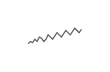
\begin{tikzpicture}[x=0.08em, y=0.08em, line width=0.4pt]
                \draw[FooterGray] (0,3) -- (1,4) -- (2,3.5) -- (3,5) -- (4,4) -- (5,6) -- (6,5.5) -- (7,4) -- (8,5) -- (9,7) -- (10,6) -- (11,5) -- (12,6.5) -- (13,8) -- (14,7) -- (15,6) -- (16,7.5) -- (17,9) -- (18,8) -- (19,7) -- (20,8.5) -- (21,10) -- (22,9) -- (23,8) -- (24,9.5);
            \end{tikzpicture}%
        }%
        \hskip0.5cm%
    }%
    \vskip6pt%
}

%=============================================================================
% PACKAGES
%=============================================================================
\usepackage[utf8]{inputenc}
\DeclareUnicodeCharacter{03B1}{\ensuremath{\alpha}}
\usepackage[T1]{fontenc}
\usepackage{amsmath, amssymb, amsthm}
\usepackage{mathtools}
\usepackage{bm}
\usepackage{tikz}
\usetikzlibrary{arrows.meta, positioning, shapes, calc, decorations.pathreplacing, shadings}
\usepackage{booktabs}
\usepackage{multirow}
\usepackage{array}
\usepackage{graphicx}
\usepackage{animate}
\usepackage{hyperref}
\usepackage{colortbl}
\usepackage{listings}
\lstset{language=Python, basicstyle=\ttfamily\scriptsize, keywordstyle=\color{MainBlue}\bfseries,
  commentstyle=\color{Forest}, stringstyle=\color{Crimson}, breaklines=true,
  frame=none, backgroundcolor=\color{VeryLightGray}, xleftmargin=2mm}
\hypersetup{colorlinks=true, linkcolor=MainBlue, urlcolor=MainBlue}
\graphicspath{{../../logos/}{../../charts/}{../../photos/}}
\usepackage{xcolor}
\hfuzz=2pt  % Suppress tiny overfull warnings (<2pt)
\vfuzz=2pt  % Suppress tiny vertical overfull warnings (<2pt)
% \mathrm in the sans-serif family of the slides (beamer resets \mathrm to the serif family at \begin{document};
% this hook runs after beamer's, so WN, Var, RMSE, ... in formulas match the surrounding text)
% Bold vectors and matrices in the same sans-serif family: \mathbf{A} in sans bold (beamer's own \mathbf came out in
% medium weight), and the bold upright Greek capitals of \boldsymbol / \bm (\bSigma, \bPhi, \boldsymbol{\Theta}) in
% cmss bold: bm.sty fixes its "boldoperators" font when it is loaded (serif cmbx), before beamer switches the
% operators to cmss, so it is reset here.
\AtBeginDocument{%
  \SetMathAlphabet{\mathrm}{normal}{\encodingdefault}{\sfdefault}{\mddefault}{n}%
  \SetMathAlphabet{\mathrm}{bold}{\encodingdefault}{\sfdefault}{bx}{n}%
  \SetMathAlphabet{\mathbf}{normal}{\encodingdefault}{\sfdefault}{bx}{n}%
  \SetMathAlphabet{\mathbf}{bold}{\encodingdefault}{\sfdefault}{bx}{n}%
  \SetSymbolFont{boldoperators}{normal}{OT1}{cmss}{bx}{n}%
  \SetSymbolFont{boldoperators}{bold}{OT1}{cmss}{bx}{n}}

%=============================================================================
% QUANTLET COMMANDS
%   \quantlet{<displayed name>}{<url>}       (generic, compatible with the older TSA decks)
%   \tsaquantlet{Ch_05}{TSA_ch5_garch}       -> https://github.com/danpele/Time-Series-Analysis/tree/main/Quantlets/Ch_05/TSA_ch5_garch
%   \qlurl{<folder>} is defined per chapter by the generator (Quantlets/Ch_NN/<folder>)
%=============================================================================
\newcommand{\tsarepo}{https://github.com/danpele/Time-Series-Analysis}
\newcommand{\tsaqlbase}{https://github.com/danpele/Time-Series-Analysis/tree/main/Quantlets}
\newcommand{\quantlet}[2]{%
    \hfill\href{#2}{%
        \raisebox{-0.15em}{
\includegraphics[height=0.7em]{ql_logo.png}}%
        \textcolor{MainBlue}{\tiny\ #1}%
    }%
}
\newcommand{\tsaquantlet}[2]{\quantlet{\detokenize{#2}}{\tsaqlbase/#1/#2}}

%=============================================================================
% NOTEBOOKS (Google Colab)
%   \colaburl{notebooks/EN/chapter5_seminar_notebook.ipynb} -> the Colab link of a file in the TSA repo
%   \nb: the chapter notebook (each seminar deck redefines it with \renewcommand)
%=============================================================================
\newcommand{\colaburl}[1]{https://colab.research.google.com/github/danpele/Time-Series-Analysis/blob/main/#1}
\newcommand{\nb}{https://colab.research.google.com/github/danpele/Time-Series-Analysis/tree/main/notebooks/EN}
\newcommand{\nbname}{notebooks/EN}

%=============================================================================
% SLIDE HELPERS (used by the generators; the same as in MFM)
%=============================================================================
% local font size for list bodies (the preamble forces \normalsize)
\newcommand{\itemsize}[1]{\setbeamertemplate{itemize/enumerate body begin}{#1}\setbeamertemplate{itemize/enumerate subbody begin}{#1}}
\newcommand{\intitle}[1]{{\hypersetup{urlcolor=white}#1}}   % white links inside coloured title bars
\newcommand{\imgcap}[1]{{\scriptsize #1}\\[0.5mm]}          % caption under a photo
\newcommand{\imgcredit}[2]{{\tiny\color{FooterGray}\href{#1}{#2}}}   % image credit: source URL, author/licence
\newcommand{\aiprompt}[1]{{\ttfamily\color{MainBlue}#1}}     % a prompt to an AI assistant

%=============================================================================
% SEMINARS: student version by default; the instructor wrapper *_solutions.tex sets \solutionstrue
%=============================================================================
\makeatletter\@ifundefined{ifsolutions}{\expandafter\newif\csname ifsolutions\endcsname}{}\makeatother
\newcommand{\solonly}[1]{\ifsolutions #1\fi}
\newcommand{\propsub}{\ifsolutions\else\framesubtitle{\ifdefined\tsalang Rezolvarea se discută la seminar\else Solution discussed in class\fi}\fi}

%=============================================================================
% APPENDIX AND CHAPTER LINKS (latex/appendix_links.py writes the calls; it also re-declares these
% macros before \begin{document}, so the decks compile with or without this preamble block)
%=============================================================================
\providecommand{\tsaapplink}[3]{\hypertarget{#2}{}\hyperlink{#1}{\beamergotobutton{#3}}}
\providecommand{\tsaappback}[2]{\begin{tikzpicture}[remember picture,overlay]\node[anchor=south east] at ([xshift=-3mm,yshift=7mm]current page.south east){\hyperlink{#1}{\beamerreturnbutton{#2}}};\end{tikzpicture}}
\providecommand{\tsachlink}[2]{\href{#1}{#2}}
\providecommand{\tsachlinkt}[2]{\href{#1}{\usebeamercolor[fg]{frametitle}#2}}

%=============================================================================
% QUANTINAR COMMAND: link către un curs Quantinar (subiecte avansate)
%=============================================================================
\newcommand{\quantinar}[2]{%
    \href{#2}{%
        \raisebox{-0.15em}{
\includegraphics[height=0.8em]{qr_logo.png}}%
        \textcolor{MainBlue}{\scriptsize\ #1}%
    }%
}

%=============================================================================
% CUSTOM TITLE PAGE
%=============================================================================
\defbeamertemplate*{title page}{hybrid}[1][]
{
    \vspace{0.2cm}
    % Logos row - top header (with clickable links)
    \begin{center}
        \href{https://www.ase.ro}{
\includegraphics[height=1.0cm]{ase_logo.png}}\hspace{0.3cm}%
        \href{https://theida.net}{
\includegraphics[height=1.0cm]{ida_logo.png}}\hspace{0.3cm}%
        \href{https://blockchain-research-center.com}{
\includegraphics[height=1.0cm]{brc_logo.png}}\hspace{0.3cm}%
        \href{https://www.ai4efin.ase.ro}{
\includegraphics[height=1.0cm]{ai4efin_logo.png}}\hspace{0.3cm}%
        \href{https://ipe.ro/new}{
\includegraphics[height=1.0cm]{acad_logo.png}}\hspace{0.3cm}%
        \href{https://www.digital-finance-msca.com}{
\includegraphics[height=1.0cm]{msca_logo.png}}%
    \end{center}

    \vspace{0.6cm}

    % Main title with Q logos on sides (with clickable links)
    \begin{center}
        \begin{minipage}{0.1\textwidth}
            \centering
            \href{https://quantlet.com}{
\includegraphics[height=1.1cm]{ql_logo.png}}
        \end{minipage}%
        \begin{minipage}{0.78\textwidth}
            \centering
            {\LARGE\bfseries\usebeamercolor[fg]{title}\inserttitle}

            \vspace{0.3cm}

            {\usebeamerfont{subtitle}\usebeamercolor[fg]{title}\insertsubtitle}
        \end{minipage}%
        \begin{minipage}{0.1\textwidth}
            \centering
            \href{https://quantinar.com}{
\includegraphics[height=1.1cm]{qr_logo.png}}
        \end{minipage}
    \end{center}

    \vspace{0.6cm}

    % Authors (left aligned)
    \hspace{0.5cm}{\usebeamerfont{author}\insertauthor}

    \vspace{0.3cm}

    % Institute/Affiliations (left aligned)
    \hspace{0.5cm}\begin{minipage}[t]{0.9\textwidth}
        \raggedright\small\insertinstitute
    \end{minipage}
}

%=============================================================================
% THEOREM ENVIRONMENTS
%=============================================================================
\theoremstyle{definition}
\setbeamertemplate{theorems}[numbered]
\ifdefined\tsalang
\newtheorem{defn}{Definiție}
\newtheorem{thm}{Teoremă}
\newtheorem{prop}{Propoziție}
\newtheorem{rmk}{Observație}
\else
\newtheorem{defn}{Definition}
\newtheorem{thm}{Theorem}
\newtheorem{prop}{Proposition}
\newtheorem{rmk}{Remark}
\fi

%=============================================================================
% CENTRED MINIPAGE (no extra vertical space)
%=============================================================================
\newenvironment{cminipage}[1]{%
    \par\noindent\hfill\begin{minipage}{#1}\ignorespaces
}{%
    \end{minipage}\hfill\null\par
}

%=============================================================================
% CUSTOM COMMANDS
%=============================================================================
\newcommand{\E}{\mathbb{E}}
\newcommand{\Var}{\text{Var}}
\newcommand{\Cov}{\text{Cov}}
\newcommand{\Corr}{\text{Corr}}
\newcommand{\R}{\mathbb{R}}
\newcommand{\N}{\mathbb{N}}
\newcommand{\Z}{\mathbb{Z}}
\newcommand{\B}{\mathbf{B}}
\newcommand{\imark}{\textcolor{MainBlue}{\textbullet}}
\newcommand{\RMSE}{\text{RMSE}}
\newcommand{\MAE}{\text{MAE}}
\newcommand{\MAPE}{\text{MAPE}}

% Boldface vector/matrix commands (VAR, VECM, state space; also used by the older TSA decks)
\newcommand{\bY}{\mathbf{Y}}
\newcommand{\bX}{\mathbf{X}}
\newcommand{\bA}{\mathbf{A}}
\newcommand{\bB}{\mathbf{B}}
\newcommand{\bepsilon}{\boldsymbol{\varepsilon}}
\newcommand{\bSigma}{\boldsymbol{\Sigma}}
\newcommand{\bPhi}{\boldsymbol{\Phi}}
\newcommand{\bGamma}{\boldsymbol{\Gamma}}
\newcommand{\bPi}{\boldsymbol{\Pi}}
\newcommand{\bc}{\mathbf{c}}
\newcommand{\balpha}{\boldsymbol{\alpha}}
\newcommand{\bbeta}{\boldsymbol{\beta}}
\newcommand{\bvarepsilon}{\boldsymbol{\varepsilon}}

% Legacy seminar marks (older TSA seminar decks)
\newcommand{\correct}{\textcolor{Forest}{\checkmark}}
\newcommand{\incorrect}{\textcolor{Crimson}{\texttimes}}
 se definește
%   \newcommand{\coursename}{Time Series Analysis}      (EN)
%   \newcommand{\coursename}{Serii de timp}       (RO)  și  \def\tsalang{ro}
% Fișierele .tex se află în EN/Courses, EN/Seminars, RO/Cursuri, RO/Seminarii (două niveluri sub rădăcină).
% Deck-urile sînt generate de latex/build_chapterN.py / build_seminarN.py (vezi latex/tsa_build.py).

\documentclass[9pt, aspectratio=169, t]{beamer}
\providecommand{\coursename}{Time Series Analysis}

% Ensure content fits on slides
\setbeamersize{text margin left=8mm, text margin right=8mm}
% Smaller institute font (title page)
\setbeamerfont{institute}{size=\footnotesize}

%=============================================================================
% THEME AND STYLE CONFIGURATION
%=============================================================================
\usetheme{default}
% Using default theme for clean header/footer control

% Color Palette (matching Redispatch PDF)
\definecolor{MainBlue}{RGB}{26, 58, 110}
\definecolor{AccentBlue}{RGB}{26, 58, 110}
\definecolor{IDAred}{RGB}{205, 0, 0}
\definecolor{DarkGray}{RGB}{51, 51, 51}
\definecolor{MediumGray}{RGB}{128, 128, 128}
\definecolor{LightGray}{RGB}{248, 248, 248}
\definecolor{VeryLightGray}{RGB}{235, 235, 235}
\definecolor{KeynoteGray}{RGB}{218, 218, 218}
\definecolor{SectionGray}{RGB}{120, 120, 120}
\definecolor{FooterGray}{RGB}{100, 100, 100}
\definecolor{Crimson}{RGB}{220, 53, 69}
\definecolor{Forest}{RGB}{46, 125, 50}
\definecolor{Amber}{RGB}{181, 133, 63}
\definecolor{Orange}{RGB}{230, 126, 34}
\definecolor{Purple}{RGB}{142, 68, 173}

% Gradient background (exact Keynote 315° gradient: white to RGB 218,218,218)
\setbeamertemplate{background}{%
    \begin{tikzpicture}[remember picture, overlay]
        \shade[shading=axis, shading angle=315,
        top color=white, bottom color=KeynoteGray]
        (current page.south west) rectangle (current page.north east);
    \end{tikzpicture}%
}
% Fallback solid color for compatibility
\setbeamercolor{background canvas}{bg=}

\setbeamercolor{palette primary}{bg=MainBlue, fg=white}
\setbeamercolor{palette secondary}{bg=MainBlue!85, fg=white}
\setbeamercolor{palette tertiary}{bg=MainBlue!70, fg=white}
\setbeamercolor{structure}{fg=MainBlue}
\setbeamercolor{title}{fg=IDAred}
\setbeamercolor{frametitle}{fg=IDAred, bg=}
\setbeamercolor{block title}{bg=MainBlue, fg=white}
\setbeamercolor{block body}{bg=VeryLightGray, fg=DarkGray}
\setbeamercolor{block title alerted}{bg=Crimson, fg=white}
\setbeamercolor{block body alerted}{bg=Crimson!8, fg=DarkGray}
\setbeamercolor{block title example}{bg=Forest, fg=white}
\setbeamercolor{block body example}{bg=Forest!8, fg=DarkGray}
\setbeamercolor{item}{fg=MainBlue}

% Footer colors (override Madrid theme blue)
\setbeamercolor{author in head/foot}{fg=FooterGray, bg=}
\setbeamercolor{title in head/foot}{fg=FooterGray, bg=}
\setbeamercolor{date in head/foot}{fg=FooterGray, bg=}
\setbeamercolor{section in head/foot}{fg=FooterGray, bg=}
\setbeamercolor{subsection in head/foot}{fg=FooterGray, bg=}

% Bullet styles (apply everywhere including blocks)
\setbeamertemplate{itemize item}{\color{MainBlue}$\boxdot$}
\setbeamertemplate{itemize subitem}{\color{MainBlue}$\blacktriangleright$}
\setbeamertemplate{itemize subsubitem}{\color{MainBlue}\tiny$\bullet$}
\setbeamertemplate{itemize/enumerate body begin}{\normalsize}
\setbeamertemplate{itemize/enumerate subbody begin}{\normalsize}

% Item spacing - compact style
\setlength{\leftmargini}{10pt}       % Level 1: minimal indent
\setlength{\leftmarginii}{10pt}      % Level 2: minimal additional indent
% Compact list spacing (zero extra space before/after lists in blocks)
\makeatletter
\def\@listi{\leftmargin\leftmargini \topsep 0pt \parsep 0pt \itemsep 0pt}
\def\@listii{\leftmargin\leftmarginii \topsep 0pt \parsep 0pt \itemsep 0pt}
\makeatother

\setbeamertemplate{navigation symbols}{}

%=============================================================================
% CUSTOM HEADLINE
%=============================================================================
\setbeamertemplate{headline}{%
    \vskip10pt%
    \hbox to \paperwidth{%
        \hskip0.5cm%
        {\small\color{FooterGray}\renewcommand{\hyperlink}[2]{##2}\insertsectionhead}%
        \hfill%
        \textcolor{FooterGray}{\small\insertframenumber}%
        \hskip0.5cm%
    }%
    \vskip4pt%
    {\color{FooterGray}\hrule height 0.4pt}%
}

%=============================================================================
% CUSTOM FOOTER
%=============================================================================
\usepackage{fontawesome5}

\setbeamertemplate{footline}{%
    {\color{FooterGray}\hrule height 0.4pt}%
    \vskip4pt%
    \hbox to \paperwidth{%
        \hskip0.5cm%
        \textcolor{FooterGray}{\small\coursename}%
        \hfill%
        \raisebox{-0.1em}{%
            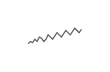
\begin{tikzpicture}[x=0.08em, y=0.08em, line width=0.4pt]
                \draw[FooterGray] (0,3) -- (1,4) -- (2,3.5) -- (3,5) -- (4,4) -- (5,6) -- (6,5.5) -- (7,4) -- (8,5) -- (9,7) -- (10,6) -- (11,5) -- (12,6.5) -- (13,8) -- (14,7) -- (15,6) -- (16,7.5) -- (17,9) -- (18,8) -- (19,7) -- (20,8.5) -- (21,10) -- (22,9) -- (23,8) -- (24,9.5);
            \end{tikzpicture}%
        }%
        \hskip0.5cm%
    }%
    \vskip6pt%
}

%=============================================================================
% PACKAGES
%=============================================================================
\usepackage[utf8]{inputenc}
\DeclareUnicodeCharacter{03B1}{\ensuremath{\alpha}}
\usepackage[T1]{fontenc}
\usepackage{amsmath, amssymb, amsthm}
\usepackage{mathtools}
\usepackage{bm}
\usepackage{tikz}
\usetikzlibrary{arrows.meta, positioning, shapes, calc, decorations.pathreplacing, shadings}
\usepackage{booktabs}
\usepackage{multirow}
\usepackage{array}
\usepackage{graphicx}
\usepackage{animate}
\usepackage{hyperref}
\usepackage{colortbl}
\usepackage{listings}
\lstset{language=Python, basicstyle=\ttfamily\scriptsize, keywordstyle=\color{MainBlue}\bfseries,
  commentstyle=\color{Forest}, stringstyle=\color{Crimson}, breaklines=true,
  frame=none, backgroundcolor=\color{VeryLightGray}, xleftmargin=2mm}
\hypersetup{colorlinks=true, linkcolor=MainBlue, urlcolor=MainBlue}
\graphicspath{{../../logos/}{../../charts/}{../../photos/}}
\usepackage{xcolor}
\hfuzz=2pt  % Suppress tiny overfull warnings (<2pt)
\vfuzz=2pt  % Suppress tiny vertical overfull warnings (<2pt)
% \mathrm in the sans-serif family of the slides (beamer resets \mathrm to the serif family at \begin{document};
% this hook runs after beamer's, so WN, Var, RMSE, ... in formulas match the surrounding text)
% Bold vectors and matrices in the same sans-serif family: \mathbf{A} in sans bold (beamer's own \mathbf came out in
% medium weight), and the bold upright Greek capitals of \boldsymbol / \bm (\bSigma, \bPhi, \boldsymbol{\Theta}) in
% cmss bold: bm.sty fixes its "boldoperators" font when it is loaded (serif cmbx), before beamer switches the
% operators to cmss, so it is reset here.
\AtBeginDocument{%
  \SetMathAlphabet{\mathrm}{normal}{\encodingdefault}{\sfdefault}{\mddefault}{n}%
  \SetMathAlphabet{\mathrm}{bold}{\encodingdefault}{\sfdefault}{bx}{n}%
  \SetMathAlphabet{\mathbf}{normal}{\encodingdefault}{\sfdefault}{bx}{n}%
  \SetMathAlphabet{\mathbf}{bold}{\encodingdefault}{\sfdefault}{bx}{n}%
  \SetSymbolFont{boldoperators}{normal}{OT1}{cmss}{bx}{n}%
  \SetSymbolFont{boldoperators}{bold}{OT1}{cmss}{bx}{n}}

%=============================================================================
% QUANTLET COMMANDS
%   \quantlet{<displayed name>}{<url>}       (generic, compatible with the older TSA decks)
%   \tsaquantlet{Ch_05}{TSA_ch5_garch}       -> https://github.com/danpele/Time-Series-Analysis/tree/main/Quantlets/Ch_05/TSA_ch5_garch
%   \qlurl{<folder>} is defined per chapter by the generator (Quantlets/Ch_NN/<folder>)
%=============================================================================
\newcommand{\tsarepo}{https://github.com/danpele/Time-Series-Analysis}
\newcommand{\tsaqlbase}{https://github.com/danpele/Time-Series-Analysis/tree/main/Quantlets}
\newcommand{\quantlet}[2]{%
    \hfill\href{#2}{%
        \raisebox{-0.15em}{
\includegraphics[height=0.7em]{ql_logo.png}}%
        \textcolor{MainBlue}{\tiny\ #1}%
    }%
}
\newcommand{\tsaquantlet}[2]{\quantlet{\detokenize{#2}}{\tsaqlbase/#1/#2}}

%=============================================================================
% NOTEBOOKS (Google Colab)
%   \colaburl{notebooks/EN/chapter5_seminar_notebook.ipynb} -> the Colab link of a file in the TSA repo
%   \nb: the chapter notebook (each seminar deck redefines it with \renewcommand)
%=============================================================================
\newcommand{\colaburl}[1]{https://colab.research.google.com/github/danpele/Time-Series-Analysis/blob/main/#1}
\newcommand{\nb}{https://colab.research.google.com/github/danpele/Time-Series-Analysis/tree/main/notebooks/EN}
\newcommand{\nbname}{notebooks/EN}

%=============================================================================
% SLIDE HELPERS (used by the generators; the same as in MFM)
%=============================================================================
% local font size for list bodies (the preamble forces \normalsize)
\newcommand{\itemsize}[1]{\setbeamertemplate{itemize/enumerate body begin}{#1}\setbeamertemplate{itemize/enumerate subbody begin}{#1}}
\newcommand{\intitle}[1]{{\hypersetup{urlcolor=white}#1}}   % white links inside coloured title bars
\newcommand{\imgcap}[1]{{\scriptsize #1}\\[0.5mm]}          % caption under a photo
\newcommand{\imgcredit}[2]{{\tiny\color{FooterGray}\href{#1}{#2}}}   % image credit: source URL, author/licence
\newcommand{\aiprompt}[1]{{\ttfamily\color{MainBlue}#1}}     % a prompt to an AI assistant

%=============================================================================
% SEMINARS: student version by default; the instructor wrapper *_solutions.tex sets \solutionstrue
%=============================================================================
\makeatletter\@ifundefined{ifsolutions}{\expandafter\newif\csname ifsolutions\endcsname}{}\makeatother
\newcommand{\solonly}[1]{\ifsolutions #1\fi}
\newcommand{\propsub}{\ifsolutions\else\framesubtitle{\ifdefined\tsalang Rezolvarea se discută la seminar\else Solution discussed in class\fi}\fi}

%=============================================================================
% APPENDIX AND CHAPTER LINKS (latex/appendix_links.py writes the calls; it also re-declares these
% macros before \begin{document}, so the decks compile with or without this preamble block)
%=============================================================================
\providecommand{\tsaapplink}[3]{\hypertarget{#2}{}\hyperlink{#1}{\beamergotobutton{#3}}}
\providecommand{\tsaappback}[2]{\begin{tikzpicture}[remember picture,overlay]\node[anchor=south east] at ([xshift=-3mm,yshift=7mm]current page.south east){\hyperlink{#1}{\beamerreturnbutton{#2}}};\end{tikzpicture}}
\providecommand{\tsachlink}[2]{\href{#1}{#2}}
\providecommand{\tsachlinkt}[2]{\href{#1}{\usebeamercolor[fg]{frametitle}#2}}

%=============================================================================
% QUANTINAR COMMAND: link către un curs Quantinar (subiecte avansate)
%=============================================================================
\newcommand{\quantinar}[2]{%
    \href{#2}{%
        \raisebox{-0.15em}{
\includegraphics[height=0.8em]{qr_logo.png}}%
        \textcolor{MainBlue}{\scriptsize\ #1}%
    }%
}

%=============================================================================
% CUSTOM TITLE PAGE
%=============================================================================
\defbeamertemplate*{title page}{hybrid}[1][]
{
    \vspace{0.2cm}
    % Logos row - top header (with clickable links)
    \begin{center}
        \href{https://www.ase.ro}{
\includegraphics[height=1.0cm]{ase_logo.png}}\hspace{0.3cm}%
        \href{https://theida.net}{
\includegraphics[height=1.0cm]{ida_logo.png}}\hspace{0.3cm}%
        \href{https://blockchain-research-center.com}{
\includegraphics[height=1.0cm]{brc_logo.png}}\hspace{0.3cm}%
        \href{https://www.ai4efin.ase.ro}{
\includegraphics[height=1.0cm]{ai4efin_logo.png}}\hspace{0.3cm}%
        \href{https://ipe.ro/new}{
\includegraphics[height=1.0cm]{acad_logo.png}}\hspace{0.3cm}%
        \href{https://www.digital-finance-msca.com}{
\includegraphics[height=1.0cm]{msca_logo.png}}%
    \end{center}

    \vspace{0.6cm}

    % Main title with Q logos on sides (with clickable links)
    \begin{center}
        \begin{minipage}{0.1\textwidth}
            \centering
            \href{https://quantlet.com}{
\includegraphics[height=1.1cm]{ql_logo.png}}
        \end{minipage}%
        \begin{minipage}{0.78\textwidth}
            \centering
            {\LARGE\bfseries\usebeamercolor[fg]{title}\inserttitle}

            \vspace{0.3cm}

            {\usebeamerfont{subtitle}\usebeamercolor[fg]{title}\insertsubtitle}
        \end{minipage}%
        \begin{minipage}{0.1\textwidth}
            \centering
            \href{https://quantinar.com}{
\includegraphics[height=1.1cm]{qr_logo.png}}
        \end{minipage}
    \end{center}

    \vspace{0.6cm}

    % Authors (left aligned)
    \hspace{0.5cm}{\usebeamerfont{author}\insertauthor}

    \vspace{0.3cm}

    % Institute/Affiliations (left aligned)
    \hspace{0.5cm}\begin{minipage}[t]{0.9\textwidth}
        \raggedright\small\insertinstitute
    \end{minipage}
}

%=============================================================================
% THEOREM ENVIRONMENTS
%=============================================================================
\theoremstyle{definition}
\setbeamertemplate{theorems}[numbered]
\ifdefined\tsalang
\newtheorem{defn}{Definiție}
\newtheorem{thm}{Teoremă}
\newtheorem{prop}{Propoziție}
\newtheorem{rmk}{Observație}
\else
\newtheorem{defn}{Definition}
\newtheorem{thm}{Theorem}
\newtheorem{prop}{Proposition}
\newtheorem{rmk}{Remark}
\fi

%=============================================================================
% CENTRED MINIPAGE (no extra vertical space)
%=============================================================================
\newenvironment{cminipage}[1]{%
    \par\noindent\hfill\begin{minipage}{#1}\ignorespaces
}{%
    \end{minipage}\hfill\null\par
}

%=============================================================================
% CUSTOM COMMANDS
%=============================================================================
\newcommand{\E}{\mathbb{E}}
\newcommand{\Var}{\text{Var}}
\newcommand{\Cov}{\text{Cov}}
\newcommand{\Corr}{\text{Corr}}
\newcommand{\R}{\mathbb{R}}
\newcommand{\N}{\mathbb{N}}
\newcommand{\Z}{\mathbb{Z}}
\newcommand{\B}{\mathbf{B}}
\newcommand{\imark}{\textcolor{MainBlue}{\textbullet}}
\newcommand{\RMSE}{\text{RMSE}}
\newcommand{\MAE}{\text{MAE}}
\newcommand{\MAPE}{\text{MAPE}}

% Boldface vector/matrix commands (VAR, VECM, state space; also used by the older TSA decks)
\newcommand{\bY}{\mathbf{Y}}
\newcommand{\bX}{\mathbf{X}}
\newcommand{\bA}{\mathbf{A}}
\newcommand{\bB}{\mathbf{B}}
\newcommand{\bepsilon}{\boldsymbol{\varepsilon}}
\newcommand{\bSigma}{\boldsymbol{\Sigma}}
\newcommand{\bPhi}{\boldsymbol{\Phi}}
\newcommand{\bGamma}{\boldsymbol{\Gamma}}
\newcommand{\bPi}{\boldsymbol{\Pi}}
\newcommand{\bc}{\mathbf{c}}
\newcommand{\balpha}{\boldsymbol{\alpha}}
\newcommand{\bbeta}{\boldsymbol{\beta}}
\newcommand{\bvarepsilon}{\boldsymbol{\varepsilon}}

% Legacy seminar marks (older TSA seminar decks)
\newcommand{\correct}{\textcolor{Forest}{\checkmark}}
\newcommand{\incorrect}{\textcolor{Crimson}{\texttimes}}
 se definește
%   \newcommand{\coursename}{Time Series Analysis}      (EN)
%   \newcommand{\coursename}{Serii de timp}       (RO)  și  \def\tsalang{ro}
% Fișierele .tex se află în EN/Courses, EN/Seminars, RO/Cursuri, RO/Seminarii (două niveluri sub rădăcină).
% Deck-urile sînt generate de latex/build_chapterN.py / build_seminarN.py (vezi latex/tsa_build.py).

\documentclass[9pt, aspectratio=169, t]{beamer}
\providecommand{\coursename}{Time Series Analysis}

% Ensure content fits on slides
\setbeamersize{text margin left=8mm, text margin right=8mm}
% Smaller institute font (title page)
\setbeamerfont{institute}{size=\footnotesize}

%=============================================================================
% THEME AND STYLE CONFIGURATION
%=============================================================================
\usetheme{default}
% Using default theme for clean header/footer control

% Color Palette (matching Redispatch PDF)
\definecolor{MainBlue}{RGB}{26, 58, 110}
\definecolor{AccentBlue}{RGB}{26, 58, 110}
\definecolor{IDAred}{RGB}{205, 0, 0}
\definecolor{DarkGray}{RGB}{51, 51, 51}
\definecolor{MediumGray}{RGB}{128, 128, 128}
\definecolor{LightGray}{RGB}{248, 248, 248}
\definecolor{VeryLightGray}{RGB}{235, 235, 235}
\definecolor{KeynoteGray}{RGB}{218, 218, 218}
\definecolor{SectionGray}{RGB}{120, 120, 120}
\definecolor{FooterGray}{RGB}{100, 100, 100}
\definecolor{Crimson}{RGB}{220, 53, 69}
\definecolor{Forest}{RGB}{46, 125, 50}
\definecolor{Amber}{RGB}{181, 133, 63}
\definecolor{Orange}{RGB}{230, 126, 34}
\definecolor{Purple}{RGB}{142, 68, 173}

% Gradient background (exact Keynote 315° gradient: white to RGB 218,218,218)
\setbeamertemplate{background}{%
    \begin{tikzpicture}[remember picture, overlay]
        \shade[shading=axis, shading angle=315,
        top color=white, bottom color=KeynoteGray]
        (current page.south west) rectangle (current page.north east);
    \end{tikzpicture}%
}
% Fallback solid color for compatibility
\setbeamercolor{background canvas}{bg=}

\setbeamercolor{palette primary}{bg=MainBlue, fg=white}
\setbeamercolor{palette secondary}{bg=MainBlue!85, fg=white}
\setbeamercolor{palette tertiary}{bg=MainBlue!70, fg=white}
\setbeamercolor{structure}{fg=MainBlue}
\setbeamercolor{title}{fg=IDAred}
\setbeamercolor{frametitle}{fg=IDAred, bg=}
\setbeamercolor{block title}{bg=MainBlue, fg=white}
\setbeamercolor{block body}{bg=VeryLightGray, fg=DarkGray}
\setbeamercolor{block title alerted}{bg=Crimson, fg=white}
\setbeamercolor{block body alerted}{bg=Crimson!8, fg=DarkGray}
\setbeamercolor{block title example}{bg=Forest, fg=white}
\setbeamercolor{block body example}{bg=Forest!8, fg=DarkGray}
\setbeamercolor{item}{fg=MainBlue}

% Footer colors (override Madrid theme blue)
\setbeamercolor{author in head/foot}{fg=FooterGray, bg=}
\setbeamercolor{title in head/foot}{fg=FooterGray, bg=}
\setbeamercolor{date in head/foot}{fg=FooterGray, bg=}
\setbeamercolor{section in head/foot}{fg=FooterGray, bg=}
\setbeamercolor{subsection in head/foot}{fg=FooterGray, bg=}

% Bullet styles (apply everywhere including blocks)
\setbeamertemplate{itemize item}{\color{MainBlue}$\boxdot$}
\setbeamertemplate{itemize subitem}{\color{MainBlue}$\blacktriangleright$}
\setbeamertemplate{itemize subsubitem}{\color{MainBlue}\tiny$\bullet$}
\setbeamertemplate{itemize/enumerate body begin}{\normalsize}
\setbeamertemplate{itemize/enumerate subbody begin}{\normalsize}

% Item spacing - compact style
\setlength{\leftmargini}{10pt}       % Level 1: minimal indent
\setlength{\leftmarginii}{10pt}      % Level 2: minimal additional indent
% Compact list spacing (zero extra space before/after lists in blocks)
\makeatletter
\def\@listi{\leftmargin\leftmargini \topsep 0pt \parsep 0pt \itemsep 0pt}
\def\@listii{\leftmargin\leftmarginii \topsep 0pt \parsep 0pt \itemsep 0pt}
\makeatother

\setbeamertemplate{navigation symbols}{}

%=============================================================================
% CUSTOM HEADLINE
%=============================================================================
\setbeamertemplate{headline}{%
    \vskip10pt%
    \hbox to \paperwidth{%
        \hskip0.5cm%
        {\small\color{FooterGray}\renewcommand{\hyperlink}[2]{##2}\insertsectionhead}%
        \hfill%
        \textcolor{FooterGray}{\small\insertframenumber}%
        \hskip0.5cm%
    }%
    \vskip4pt%
    {\color{FooterGray}\hrule height 0.4pt}%
}

%=============================================================================
% CUSTOM FOOTER
%=============================================================================
\usepackage{fontawesome5}

\setbeamertemplate{footline}{%
    {\color{FooterGray}\hrule height 0.4pt}%
    \vskip4pt%
    \hbox to \paperwidth{%
        \hskip0.5cm%
        \textcolor{FooterGray}{\small\coursename}%
        \hfill%
        \raisebox{-0.1em}{%
            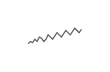
\begin{tikzpicture}[x=0.08em, y=0.08em, line width=0.4pt]
                \draw[FooterGray] (0,3) -- (1,4) -- (2,3.5) -- (3,5) -- (4,4) -- (5,6) -- (6,5.5) -- (7,4) -- (8,5) -- (9,7) -- (10,6) -- (11,5) -- (12,6.5) -- (13,8) -- (14,7) -- (15,6) -- (16,7.5) -- (17,9) -- (18,8) -- (19,7) -- (20,8.5) -- (21,10) -- (22,9) -- (23,8) -- (24,9.5);
            \end{tikzpicture}%
        }%
        \hskip0.5cm%
    }%
    \vskip6pt%
}

%=============================================================================
% PACKAGES
%=============================================================================
\usepackage[utf8]{inputenc}
\DeclareUnicodeCharacter{03B1}{\ensuremath{\alpha}}
\usepackage[T1]{fontenc}
\usepackage{amsmath, amssymb, amsthm}
\usepackage{mathtools}
\usepackage{bm}
\usepackage{tikz}
\usetikzlibrary{arrows.meta, positioning, shapes, calc, decorations.pathreplacing, shadings}
\usepackage{booktabs}
\usepackage{multirow}
\usepackage{array}
\usepackage{graphicx}
\usepackage{animate}
\usepackage{hyperref}
\usepackage{colortbl}
\usepackage{listings}
\lstset{language=Python, basicstyle=\ttfamily\scriptsize, keywordstyle=\color{MainBlue}\bfseries,
  commentstyle=\color{Forest}, stringstyle=\color{Crimson}, breaklines=true,
  frame=none, backgroundcolor=\color{VeryLightGray}, xleftmargin=2mm}
\hypersetup{colorlinks=true, linkcolor=MainBlue, urlcolor=MainBlue}
\graphicspath{{../../logos/}{../../charts/}{../../photos/}}
\usepackage{xcolor}
\hfuzz=2pt  % Suppress tiny overfull warnings (<2pt)
\vfuzz=2pt  % Suppress tiny vertical overfull warnings (<2pt)
% \mathrm in the sans-serif family of the slides (beamer resets \mathrm to the serif family at \begin{document};
% this hook runs after beamer's, so WN, Var, RMSE, ... in formulas match the surrounding text)
% Bold vectors and matrices in the same sans-serif family: \mathbf{A} in sans bold (beamer's own \mathbf came out in
% medium weight), and the bold upright Greek capitals of \boldsymbol / \bm (\bSigma, \bPhi, \boldsymbol{\Theta}) in
% cmss bold: bm.sty fixes its "boldoperators" font when it is loaded (serif cmbx), before beamer switches the
% operators to cmss, so it is reset here.
\AtBeginDocument{%
  \SetMathAlphabet{\mathrm}{normal}{\encodingdefault}{\sfdefault}{\mddefault}{n}%
  \SetMathAlphabet{\mathrm}{bold}{\encodingdefault}{\sfdefault}{bx}{n}%
  \SetMathAlphabet{\mathbf}{normal}{\encodingdefault}{\sfdefault}{bx}{n}%
  \SetMathAlphabet{\mathbf}{bold}{\encodingdefault}{\sfdefault}{bx}{n}%
  \SetSymbolFont{boldoperators}{normal}{OT1}{cmss}{bx}{n}%
  \SetSymbolFont{boldoperators}{bold}{OT1}{cmss}{bx}{n}}

%=============================================================================
% QUANTLET COMMANDS
%   \quantlet{<displayed name>}{<url>}       (generic, compatible with the older TSA decks)
%   \tsaquantlet{Ch_05}{TSA_ch5_garch}       -> https://github.com/danpele/Time-Series-Analysis/tree/main/Quantlets/Ch_05/TSA_ch5_garch
%   \qlurl{<folder>} is defined per chapter by the generator (Quantlets/Ch_NN/<folder>)
%=============================================================================
\newcommand{\tsarepo}{https://github.com/danpele/Time-Series-Analysis}
\newcommand{\tsaqlbase}{https://github.com/danpele/Time-Series-Analysis/tree/main/Quantlets}
\newcommand{\quantlet}[2]{%
    \hfill\href{#2}{%
        \raisebox{-0.15em}{
\includegraphics[height=0.7em]{ql_logo.png}}%
        \textcolor{MainBlue}{\tiny\ #1}%
    }%
}
\newcommand{\tsaquantlet}[2]{\quantlet{\detokenize{#2}}{\tsaqlbase/#1/#2}}

%=============================================================================
% NOTEBOOKS (Google Colab)
%   \colaburl{notebooks/EN/chapter5_seminar_notebook.ipynb} -> the Colab link of a file in the TSA repo
%   \nb: the chapter notebook (each seminar deck redefines it with \renewcommand)
%=============================================================================
\newcommand{\colaburl}[1]{https://colab.research.google.com/github/danpele/Time-Series-Analysis/blob/main/#1}
\newcommand{\nb}{https://colab.research.google.com/github/danpele/Time-Series-Analysis/tree/main/notebooks/EN}
\newcommand{\nbname}{notebooks/EN}

%=============================================================================
% SLIDE HELPERS (used by the generators; the same as in MFM)
%=============================================================================
% local font size for list bodies (the preamble forces \normalsize)
\newcommand{\itemsize}[1]{\setbeamertemplate{itemize/enumerate body begin}{#1}\setbeamertemplate{itemize/enumerate subbody begin}{#1}}
\newcommand{\intitle}[1]{{\hypersetup{urlcolor=white}#1}}   % white links inside coloured title bars
\newcommand{\imgcap}[1]{{\scriptsize #1}\\[0.5mm]}          % caption under a photo
\newcommand{\imgcredit}[2]{{\tiny\color{FooterGray}\href{#1}{#2}}}   % image credit: source URL, author/licence
\newcommand{\aiprompt}[1]{{\ttfamily\color{MainBlue}#1}}     % a prompt to an AI assistant

%=============================================================================
% SEMINARS: student version by default; the instructor wrapper *_solutions.tex sets \solutionstrue
%=============================================================================
\makeatletter\@ifundefined{ifsolutions}{\expandafter\newif\csname ifsolutions\endcsname}{}\makeatother
\newcommand{\solonly}[1]{\ifsolutions #1\fi}
\newcommand{\propsub}{\ifsolutions\else\framesubtitle{\ifdefined\tsalang Rezolvarea se discută la seminar\else Solution discussed in class\fi}\fi}

%=============================================================================
% APPENDIX AND CHAPTER LINKS (latex/appendix_links.py writes the calls; it also re-declares these
% macros before \begin{document}, so the decks compile with or without this preamble block)
%=============================================================================
\providecommand{\tsaapplink}[3]{\hypertarget{#2}{}\hyperlink{#1}{\beamergotobutton{#3}}}
\providecommand{\tsaappback}[2]{\begin{tikzpicture}[remember picture,overlay]\node[anchor=south east] at ([xshift=-3mm,yshift=7mm]current page.south east){\hyperlink{#1}{\beamerreturnbutton{#2}}};\end{tikzpicture}}
\providecommand{\tsachlink}[2]{\href{#1}{#2}}
\providecommand{\tsachlinkt}[2]{\href{#1}{\usebeamercolor[fg]{frametitle}#2}}

%=============================================================================
% QUANTINAR COMMAND: link către un curs Quantinar (subiecte avansate)
%=============================================================================
\newcommand{\quantinar}[2]{%
    \href{#2}{%
        \raisebox{-0.15em}{
\includegraphics[height=0.8em]{qr_logo.png}}%
        \textcolor{MainBlue}{\scriptsize\ #1}%
    }%
}

%=============================================================================
% CUSTOM TITLE PAGE
%=============================================================================
\defbeamertemplate*{title page}{hybrid}[1][]
{
    \vspace{0.2cm}
    % Logos row - top header (with clickable links)
    \begin{center}
        \href{https://www.ase.ro}{
\includegraphics[height=1.0cm]{ase_logo.png}}\hspace{0.3cm}%
        \href{https://theida.net}{
\includegraphics[height=1.0cm]{ida_logo.png}}\hspace{0.3cm}%
        \href{https://blockchain-research-center.com}{
\includegraphics[height=1.0cm]{brc_logo.png}}\hspace{0.3cm}%
        \href{https://www.ai4efin.ase.ro}{
\includegraphics[height=1.0cm]{ai4efin_logo.png}}\hspace{0.3cm}%
        \href{https://ipe.ro/new}{
\includegraphics[height=1.0cm]{acad_logo.png}}\hspace{0.3cm}%
        \href{https://www.digital-finance-msca.com}{
\includegraphics[height=1.0cm]{msca_logo.png}}%
    \end{center}

    \vspace{0.6cm}

    % Main title with Q logos on sides (with clickable links)
    \begin{center}
        \begin{minipage}{0.1\textwidth}
            \centering
            \href{https://quantlet.com}{
\includegraphics[height=1.1cm]{ql_logo.png}}
        \end{minipage}%
        \begin{minipage}{0.78\textwidth}
            \centering
            {\LARGE\bfseries\usebeamercolor[fg]{title}\inserttitle}

            \vspace{0.3cm}

            {\usebeamerfont{subtitle}\usebeamercolor[fg]{title}\insertsubtitle}
        \end{minipage}%
        \begin{minipage}{0.1\textwidth}
            \centering
            \href{https://quantinar.com}{
\includegraphics[height=1.1cm]{qr_logo.png}}
        \end{minipage}
    \end{center}

    \vspace{0.6cm}

    % Authors (left aligned)
    \hspace{0.5cm}{\usebeamerfont{author}\insertauthor}

    \vspace{0.3cm}

    % Institute/Affiliations (left aligned)
    \hspace{0.5cm}\begin{minipage}[t]{0.9\textwidth}
        \raggedright\small\insertinstitute
    \end{minipage}
}

%=============================================================================
% THEOREM ENVIRONMENTS
%=============================================================================
\theoremstyle{definition}
\setbeamertemplate{theorems}[numbered]
\ifdefined\tsalang
\newtheorem{defn}{Definiție}
\newtheorem{thm}{Teoremă}
\newtheorem{prop}{Propoziție}
\newtheorem{rmk}{Observație}
\else
\newtheorem{defn}{Definition}
\newtheorem{thm}{Theorem}
\newtheorem{prop}{Proposition}
\newtheorem{rmk}{Remark}
\fi

%=============================================================================
% CENTRED MINIPAGE (no extra vertical space)
%=============================================================================
\newenvironment{cminipage}[1]{%
    \par\noindent\hfill\begin{minipage}{#1}\ignorespaces
}{%
    \end{minipage}\hfill\null\par
}

%=============================================================================
% CUSTOM COMMANDS
%=============================================================================
\newcommand{\E}{\mathbb{E}}
\newcommand{\Var}{\text{Var}}
\newcommand{\Cov}{\text{Cov}}
\newcommand{\Corr}{\text{Corr}}
\newcommand{\R}{\mathbb{R}}
\newcommand{\N}{\mathbb{N}}
\newcommand{\Z}{\mathbb{Z}}
\newcommand{\B}{\mathbf{B}}
\newcommand{\imark}{\textcolor{MainBlue}{\textbullet}}
\newcommand{\RMSE}{\text{RMSE}}
\newcommand{\MAE}{\text{MAE}}
\newcommand{\MAPE}{\text{MAPE}}

% Boldface vector/matrix commands (VAR, VECM, state space; also used by the older TSA decks)
\newcommand{\bY}{\mathbf{Y}}
\newcommand{\bX}{\mathbf{X}}
\newcommand{\bA}{\mathbf{A}}
\newcommand{\bB}{\mathbf{B}}
\newcommand{\bepsilon}{\boldsymbol{\varepsilon}}
\newcommand{\bSigma}{\boldsymbol{\Sigma}}
\newcommand{\bPhi}{\boldsymbol{\Phi}}
\newcommand{\bGamma}{\boldsymbol{\Gamma}}
\newcommand{\bPi}{\boldsymbol{\Pi}}
\newcommand{\bc}{\mathbf{c}}
\newcommand{\balpha}{\boldsymbol{\alpha}}
\newcommand{\bbeta}{\boldsymbol{\beta}}
\newcommand{\bvarepsilon}{\boldsymbol{\varepsilon}}

% Legacy seminar marks (older TSA seminar decks)
\newcommand{\correct}{\textcolor{Forest}{\checkmark}}
\newcommand{\incorrect}{\textcolor{Crimson}{\texttimes}}


\newcommand{\qlurl}[1]{https://github.com/danpele/Time-Series-Analysis/tree/main/Quantlets/Ch_03/#1}

% Clickable citations (DOIs verified via Crossref)
\newcommand{\refHP}{\href{https://doi.org/10.1007/978-3-031-13584-2}{Huang and Petukhina (2022)}}
\newcommand{\refFPP}{\href{https://otexts.com/fpp3/}{Hyndman and Athanasopoulos (2021)}}
\newcommand{\refBD}{\href{https://doi.org/10.1007/978-3-319-29854-2}{Brockwell and Davis (2016)}}
\newcommand{\refHamilton}{\href{https://doi.org/10.2307/j.ctv14jx6sm}{Hamilton (1994)}}
\newcommand{\refBJ}{\href{https://doi.org/10.1002/9781118619193}{Box, Jenkins and Reinsel (2008)}}
\newcommand{\refDF}{\href{https://doi.org/10.1080/01621459.1979.10482531}{Dickey and Fuller (1979)}}
\newcommand{\refDFb}{\href{https://doi.org/10.2307/1912517}{Dickey and Fuller (1981)}}
\newcommand{\refFuller}{\href{https://doi.org/10.1002/9780470316917}{Fuller (1996)}}
\newcommand{\refSD}{\href{https://doi.org/10.1093/biomet/71.3.599}{Said and Dickey (1984)}}
\newcommand{\refPP}{\href{https://doi.org/10.1093/biomet/75.2.335}{Phillips and Perron (1988)}}
\newcommand{\refKPSS}{\href{https://doi.org/10.1016/0304-4076(92)90104-Y}{Kwiatkowski et al.\ (1992)}}
\newcommand{\refMacKinnon}{\href{https://doi.org/10.1080/07350015.1994.10510005}{MacKinnon (1994)}}
\newcommand{\refMacKinnonb}{\href{https://ideas.repec.org/p/qed/wpaper/1227.html}{MacKinnon (2010)}}
\newcommand{\refGN}{\href{https://doi.org/10.1016/0304-4076(74)90034-7}{Granger and Newbold (1974)}}
\newcommand{\refPhillips}{\href{https://doi.org/10.1016/0304-4076(86)90001-1}{Phillips (1986)}}
\newcommand{\refYule}{\href{https://doi.org/10.2307/2341482}{Yule (1926)}}
\newcommand{\refNP}{\href{https://doi.org/10.1016/0304-3932(82)90012-5}{Nelson and Plosser (1982)}}
\newcommand{\refNK}{\href{https://doi.org/10.2307/1911520}{Nelson and Kang (1981)}}
\newcommand{\refPerron}{\href{https://doi.org/10.2307/1913712}{Perron (1989)}}
\newcommand{\refZA}{\href{https://doi.org/10.1080/07350015.1992.10509904}{Zivot and Andrews (1992)}}
\newcommand{\refBaiP}{\href{https://doi.org/10.2307/2998540}{Bai and Perron (1998)}}
\newcommand{\refSchwert}{\href{https://doi.org/10.1080/07350015.1989.10509723}{Schwert (1989)}}
\newcommand{\refNgP}{\href{https://doi.org/10.1111/1468-0262.00256}{Ng and Perron (2001)}}
\newcommand{\refERS}{\href{https://doi.org/10.2307/2171846}{Elliott, Rothenberg and Stock (1996)}}
\newcommand{\refDP}{\href{https://doi.org/10.1080/07350015.1987.10509614}{Dickey and Pantula (1987)}}
\newcommand{\refPS}{\href{https://doi.org/10.1016/0304-4076(77)90015-x}{Plosser and Schwert (1977)}}
\newcommand{\refHK}{\href{https://doi.org/10.18637/jss.v027.i03}{Hyndman and Khandakar (2008)}}
\newcommand{\refMR}{\href{https://doi.org/10.1016/0022-1996(83)90017-X}{Meese and Rogoff (1983)}}
\newcommand{\refEG}{\href{https://doi.org/10.2307/1913236}{Engle and Granger (1987)}}
\newcommand{\refLB}{\href{https://doi.org/10.1093/biomet/65.2.297}{Ljung and Box (1978)}}

\title[Time Series Analysis]{Time Series Analysis}
\subtitle{Chapter 3: Unit roots and ARIMA models}
\author[D.T. Pele]{Daniel Traian PELE}
\institute{Bucharest University of Economic Studies\\
IDA Institute Digital Assets\\
Blockchain Research Center\\
AI4EFin Artificial Intelligence for Energy Finance\\
Romanian Academy, Institute for Economic Forecasting\\
MSCA Digital Finance}
\date{}

%=============================================================================
\providecommand{\tsaapplink}[3]{\hypertarget{#2}{}\hyperlink{#1}{\beamergotobutton{#3}}}  % APPLINKS-MACROS
\providecommand{\tsaappback}[2]{\begin{tikzpicture}[remember picture,overlay]\node[anchor=south east] at ([xshift=-3mm,yshift=7mm]current page.south east){\hyperlink{#1}{\beamerreturnbutton{#2}}};\end{tikzpicture}}  % APPLINKS-MACROS
\providecommand{\tsachlink}[2]{\href{#1}{#2}}  % APPLINKS-MACROS
\providecommand{\tsachlinkt}[2]{\href{#1}{\usebeamercolor[fg]{frametitle}#2}}  % APPLINKS-MACROS
\begin{document}
%=============================================================================

{
\setbeamertemplate{headline}{}
\setbeamertemplate{footline}{}
\begin{frame}[noframenumbering]
    \titlepage
\end{frame}
}
% BEGIN-ACRONYMS (generat de latex/acronyms.py; nu editati manual)
\begin{frame}{Acronyms used in this material (1/2)}
\setbeamertemplate{itemize/enumerate body begin}{\footnotesize}
\begin{columns}[T]
\begin{column}{0.49\textwidth}
\begin{itemize}\setlength{\itemsep}{0pt}
    \item \textbf{ACF}: Autocorrelation Function
    \item \textbf{ADF}: Augmented Dickey–Fuller (test)
    \item \textbf{AI}: Artificial Intelligence
    \item \textbf{AIC}: Akaike Information Criterion
    \item \textbf{AR}: AutoRegressive (model)
    \item \textbf{ARIMA}: AutoRegressive Integrated Moving Average (model)
    \item \textbf{ARMA}: AutoRegressive Moving Average (model)
    \item \textbf{BET}: Bucharest Exchange Trading (index)
    \item \textbf{BIC}: Bayesian Information Criterion
\end{itemize}
\end{column}
\begin{column}{0.49\textwidth}
\begin{itemize}\setlength{\itemsep}{0pt}
    \item \textbf{BNR}: Banca Națională a României (the National Bank of Romania)
    \item \textbf{CUSUM}: CUmulative SUM (control chart)
    \item \textbf{DF}: Dickey–Fuller (test)
    \item \textbf{DF-GLS}: Dickey–Fuller test with GLS detrending
    \item \textbf{DS}: Difference-Stationary (series)
    \item \textbf{DW}: Durbin–Watson (statistic)
    \item \textbf{EU}: European Union
    \item \textbf{FRED}: Federal Reserve Economic Data
\end{itemize}
\end{column}
\end{columns}
\end{frame}
\begin{frame}{Acronyms used in this material (2/2)}
\setbeamertemplate{itemize/enumerate body begin}{\footnotesize}
\begin{columns}[T]
\begin{column}{0.49\textwidth}
\begin{itemize}\setlength{\itemsep}{0pt}
    \item \textbf{GDP}: Gross Domestic Product
    \item \textbf{GLS}: Generalised Least Squares
    \item \textbf{GNP}: Gross National Product
    \item \textbf{HICP}: Harmonised Index of Consumer Prices
    \item \textbf{KPSS}: Kwiatkowski–Phillips–Schmidt–Shin (test)
    \item \textbf{MA}: Moving Average
    \item \textbf{MAIC}: Modified Akaike Information Criterion
    \item \textbf{OLS}: Ordinary Least Squares
    \item \textbf{PACF}: Partial AutoCorrelation Function
\end{itemize}
\end{column}
\begin{column}{0.49\textwidth}
\begin{itemize}\setlength{\itemsep}{0pt}
    \item \textbf{PP}: Phillips–Perron (test)
    \item \textbf{RMSE}: Root Mean Squared Error
    \item \textbf{SARIMA}: Seasonal ARIMA (model)
    \item \textbf{SE}: Standard Error
    \item \textbf{TBATS}: Trigonometric seasonality, Box–Cox, ARMA errors, Trend, Seasonal components (model)
    \item \textbf{TS}: Trend-Stationary (series)
    \item \textbf{US}: United States
    \item \textbf{VAR}: Vector AutoRegression
    \item \textbf{ZA}: Zivot–Andrews (test)
\end{itemize}
\end{column}
\end{columns}
\end{frame}
% END-ACRONYMS

\begin{frame}{Today's question and route}
\itemsize{\small}
\begin{itemize}
    \item \textbf{Question}: when a series drifts upwards, is the shock of today temporary or permanent, and how should we forecast it?
    \begin{itemize}
        \item the answer decides whether we detrend or difference, and how wide our forecast intervals are
    \end{itemize}
    \item \textbf{Route} of the chapter
    \begin{itemize}
        \item deterministic and stochastic trends; integrated processes $I(d)$; spurious regression
        \item unit-root tests: Dickey--Fuller, ADF, Phillips--Perron; the KPSS stationarity test; structural breaks
        \item ARIMA$(p,d,q)$ models: identification, estimation, diagnostics, forecasts with growing intervals
    \end{itemize}
    \item We build on \tsachlink{https://danpele.github.io/Time-Series-Analysis/EN/Courses/chapter1_stochastic_processes_stationarity.pdf}{Chapter 1} (stationarity, random walk, differencing) and \tsachlink{https://danpele.github.io/Time-Series-Analysis/EN/Courses/chapter2_arma_models.pdf}{Chapter 2} (ARMA models); Seminar 3 comes before this lecture
\end{itemize}
\end{frame}

\begin{frame}{Learning outcomes}
\itemsize{\small}
\begin{itemize}
    \item Distinguish trend-stationary from difference-stationary series, and explain why the distinction matters
    \item Recognise a spurious regression and explain why it happens
    \item Run and interpret the ADF, Phillips--Perron and KPSS tests, with the right deterministic terms and lags
    \item Explain how a structural break can mimic a unit root
    \item Identify, estimate, check and forecast an ARIMA$(p,d,q)$ model, and explain why its intervals grow with the horizon
    \item Use automatic ARIMA selection critically
\end{itemize}
\end{frame}

\begin{frame}{Reading and tools}
\itemsize{\small}
\begin{itemize}
    \item Textbook: \refHP, Ch.~4--5 (ARIMA models and non-stationarity)
    \begin{itemize}
        \item companion, free online: \refFPP, Ch.~9 (ARIMA models)
    \end{itemize}
    \item Theory: \refHamilton, Ch.~15--17 (trends, unit roots); \refBJ\ for the ARIMA methodology
    \item Python Quantlets of this chapter: \href{https://github.com/danpele/Time-Series-Analysis/tree/main/Quantlets/Ch_03}{Quantlets/Ch\_03}
    \begin{itemize}
        \item \texttt{adfuller}, \texttt{kpss}, \texttt{zivot\_andrews} and \texttt{ARIMA} from \texttt{statsmodels}; the Phillips--Perron test written out in a few lines
    \end{itemize}
    \item Lecture notebook: \href{\colaburl{notebooks/EN/chapter3_lecture_notebook.ipynb}}{open in Google Colab}
    \item Video course: \quantinar{Applied Time Series Analysis with Python}{https://quantinar.com/course/137/applied-time-series-analysis-with-python}
\end{itemize}
\end{frame}


%=============================================================================
\section{Deterministic and stochastic trends}
%=============================================================================

\begin{frame}{Four series that drift}
\itemsize{\footnotesize}
\begin{center}
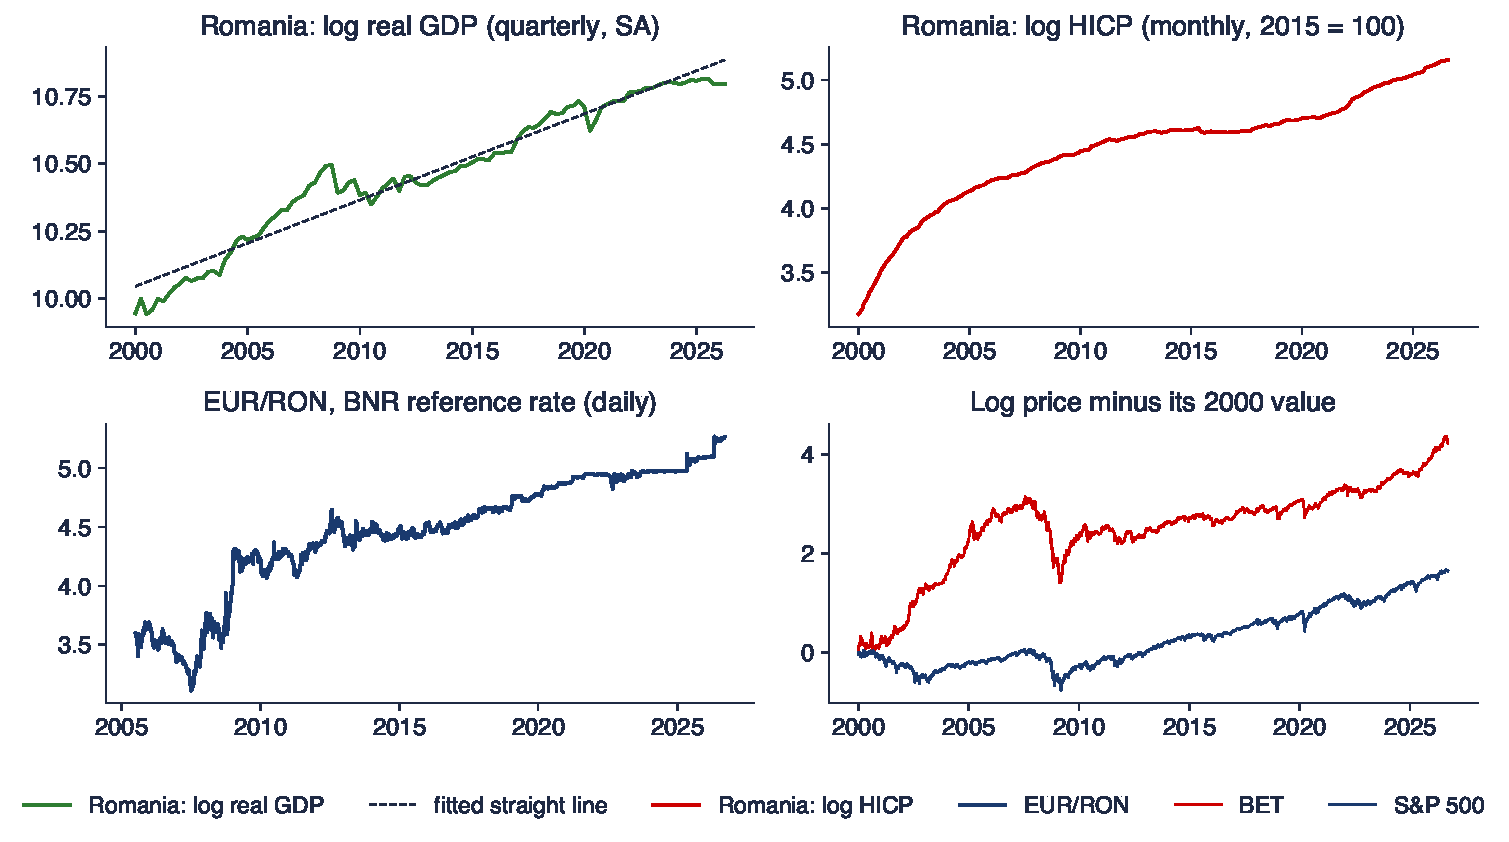
\includegraphics[width=0.97\textwidth,height=0.66\textheight,keepaspectratio]{tsa_ch3_four_series.pdf}
\end{center}
\vspace{-0.25cm}
\begin{itemize}
    \item Romanian real GDP (Eurostat, seasonally adjusted) and HICP (Eurostat); EUR/RON, the BNR reference rate; BET and S\&P 500 log prices, daily since 2000
    \item None of them has a constant mean: \tsachlink{https://danpele.github.io/Time-Series-Analysis/EN/Courses/chapter1_stochastic_processes_stationarity.pdf}{Chapter 1} called them non-stationary
\end{itemize}
\quantlet{TSA\_ch3\_trends}{\qlurl{TSA_ch3_trends}}
\end{frame}

\begin{frame}{Interpreting the four series}
\itemsize{\small}
\begin{itemize}
    \item GDP grows by 0.80\% per quarter on average (about 3.2\% per year), but it strays from the straight line by up to 18\%
    \begin{itemize}
        \item the 2009 recession: did GDP come back to the old line, or did it start a new one?
    \end{itemize}
    \item Consumer prices: $\times$7.2 since 2000; EUR/RON: from 3.60 to 5.26 lei; BET: $+426$ log points, S\&P 500: $+166$ log points (to 18 September 2026)
    \item Two models can produce such pictures
    \begin{itemize}
        \item a fixed line plus stationary noise (\textbf{deterministic trend})
        \item a random walk with drift (\textbf{stochastic trend})
    \end{itemize}
\end{itemize}
\end{frame}

\begin{frame}{Trend-stationary series}
\itemsize{\small}
\begin{itemize}
    \item \textbf{Definition}: $y_t = \alpha + \beta t + u_t$, with $u_t$ a stationary process (for example a stationary AR(1), \tsachlink{https://danpele.github.io/Time-Series-Analysis/EN/Courses/chapter2_arma_models.pdf}{Chapter 2})
    \begin{itemize}
        \item $\alpha$: the intercept; $\beta$: the slope, the average change per period; $t$: the time index
        \item $y_t$ is \textbf{trend-stationary} (TS): stationary after subtracting the line $\alpha + \beta t$
    \end{itemize}
    \item Properties
    \begin{itemize}
        \item $E[y_t] = \alpha + \beta t$; $\mathrm{Var}(y_t) = \mathrm{Var}(u_t)$, constant
        \item a shock moves $y_t$ away from the line only temporarily: with $u_t = \phi u_{t-1} + \varepsilon_t$, its effect after $h$ periods is $\phi^h$
        \item long-run forecasts return to the line; their intervals have a bounded width
    \end{itemize}
    \item Right treatment: estimate the trend by OLS (ordinary least squares) and model the residuals as ARMA
\end{itemize}
\end{frame}

\begin{frame}{Difference-stationary series}
\itemsize{\small}
\begin{itemize}
    \item \textbf{Definition}: $y_t = \beta + y_{t-1} + u_t$, $u_t$ stationary; by substitution, $y_t = y_0 + \beta t + \sum_{i=1}^{t} u_i$
    \begin{itemize}
        \item $\beta$: the drift, the average change per period; $y_0$: the starting value
        \item $y_t$ is \textbf{difference-stationary} (DS): $\Delta y_t = \beta + u_t$ is stationary
        \item $\sum_{i \le t} u_i$ is the \textbf{stochastic trend}; $\beta t$ is the drift
    \end{itemize}
    \item Properties
    \begin{itemize}
        \item the same mean $y_0 + \beta t$ as a TS series, but $\mathrm{Var}(y_t)$ grows with $t$ (\tsachlink{https://danpele.github.io/Time-Series-Analysis/EN/Courses/chapter1_stochastic_processes_stationarity.pdf}{Chapter 1}: $t\sigma^2$ for a random walk)
        \item every shock stays in the level forever: there is no line to return to
        \item forecast intervals widen without limit as the horizon grows
    \end{itemize}
    \item Right treatment: difference the series and model $\Delta y_t$ as ARMA: the ARIMA model of this chapter
\end{itemize}
\end{frame}

\begin{frame}{Same drift, different memory}
\itemsize{\footnotesize}
\begin{center}
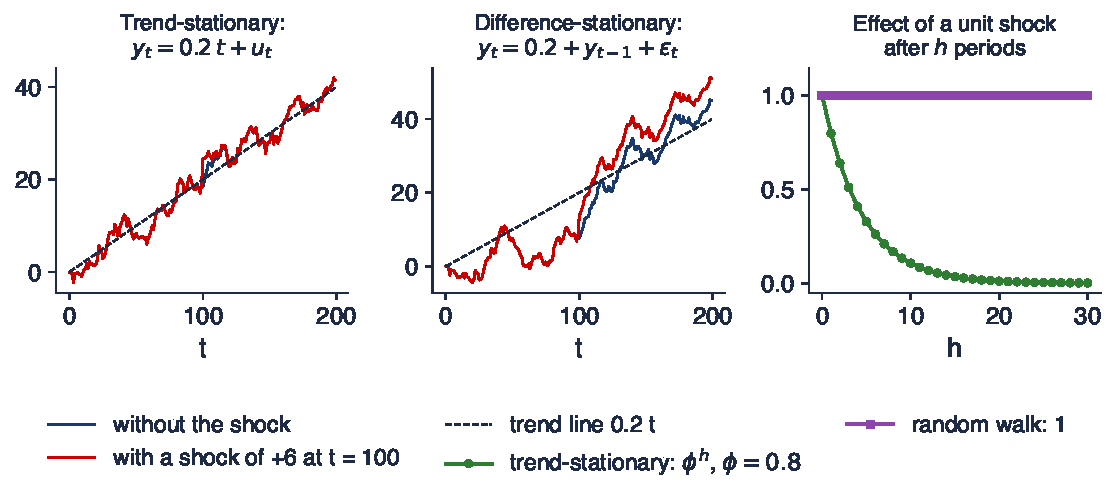
\includegraphics[width=0.97\textwidth,height=0.54\textheight,keepaspectratio]{tsa_ch3_ts_ds.pdf}
\end{center}
\vspace{-0.25cm}
\begin{itemize}
    \item Left and centre: the same shocks drive a TS series ($u_t$ AR(1), $\phi = 0.8$) and a random walk with drift 0.2; the red paths add one shock of $+6$ at $t = 100$
    \item Right: the effect of a unit shock after $h$ periods
\end{itemize}
\quantlet{TSA\_ch3\_trends}{\qlurl{TSA_ch3_trends}}
\end{frame}

\begin{frame}{Interpreting the two trends}
\itemsize{\small}
\begin{itemize}
    \item TS series: the shock dies out; its effect is $0.8^{10} = 0.107$ after 10 periods and $0.012$ after 20
    \begin{itemize}
        \item at $t = 200$ the two red and blue paths coincide
    \end{itemize}
    \item Random walk: the whole path shifts up by 6 and stays there
    \begin{itemize}
        \item a recession in a DS economy is a permanent loss of output, not a dip below a trend
    \end{itemize}
    \item By eye, the two series without the shock look alike: we need a formal test (Sections 3--4)
\end{itemize}
\end{frame}

\begin{frame}{Integrated processes}
\itemsize{\small}
\begin{itemize}
    \item \textbf{Definition}: $y_t$ is \textbf{integrated of order $d$}, $y_t \sim I(d)$, if $\Delta^d y_t$ is stationary and $\Delta^{d-1}y_t$ is not
    \begin{itemize}
        \item $I(0)$: stationary (with an invertible ARMA representation, \tsachlink{https://danpele.github.io/Time-Series-Analysis/EN/Courses/chapter2_arma_models.pdf}{Chapter 2}); $I(1)$: stationary after one difference; $I(2)$: after two
        \item $\Delta^2 y_t = \Delta y_t - \Delta y_{t-1} = y_t - 2y_{t-1} + y_{t-2}$
    \end{itemize}
    \item Typical orders in economics and finance
    \begin{itemize}
        \item log prices of stocks, exchange rates, log GDP: $I(1)$; returns and growth rates: $I(0)$
        \item price levels in high-inflation periods: possibly $I(2)$, so that inflation itself is $I(1)$
    \end{itemize}
    \item Rules
    \begin{itemize}
        \item $I(0) + I(1) = I(1)$: the stochastic trend dominates; a TS series is $I(0)$ after removing the trend, not after differencing
    \end{itemize}
\end{itemize}
\end{frame}

\begin{frame}{The unit root}
\itemsize{\small}
\begin{itemize}
    \item Write an AR($p$) with the lag operator $L$ (\tsachlink{https://danpele.github.io/Time-Series-Analysis/EN/Courses/chapter1_stochastic_processes_stationarity.pdf}{Chapter 1}): $\phi(L)y_t = \varepsilon_t$, $\phi(z) = 1 - \phi_1 z - \dots - \phi_p z^p$
    \begin{itemize}
        \item \tsachlink{https://danpele.github.io/Time-Series-Analysis/EN/Courses/chapter2_arma_models.pdf}{Chapter 2}: stationary if all roots of $\phi(z) = 0$ lie outside the unit circle, $|z| > 1$
    \end{itemize}
    \item \textbf{Unit root}: one root equals $z = 1$, so $\phi(z) = (1 - z)\,\phi^*(z)$ with the roots of $\phi^*$ outside the circle
    \begin{itemize}
        \item then $\phi^*(L)\,\Delta y_t = \varepsilon_t$: $\Delta y_t$ is a stationary AR($p-1$), and $y_t \sim I(1)$
        \item AR(1): $\phi(z) = 1 - \phi z$ has the root $1/\phi$, a unit root when $\phi = 1$: the random walk
    \end{itemize}
    \item \textbf{Example}: $y_t = 1.5y_{t-1} - 0.5y_{t-2} + \varepsilon_t$; $1 - 1.5z + 0.5z^2 = (1 - z)(1 - 0.5z)$
    \begin{itemize}
        \item roots 1 and 2: $\Delta y_t = 0.5\,\Delta y_{t-1} + \varepsilon_t$, an AR(1) in differences
    \end{itemize}
\end{itemize}
\end{frame}

\begin{frame}{Case study: Nelson and Plosser (1982)}
\itemsize{\small}
\begin{itemize}
    \item \textbf{Question}: are US macroeconomic series stationary around a trend, as the business-cycle models of the 1970s assumed?
    \begin{itemize}
        \item \refNP: 14 long annual series (real GNP, employment, prices, wages, interest rates, stock prices), some since 1860
    \end{itemize}
    \item \textbf{Method}: the Dickey--Fuller test of Section 3, with a constant and a trend
    \begin{itemize}
        \item the unit root was rejected for one series only, the unemployment rate
    \end{itemize}
    \item \textbf{Consequence}: shocks to output look permanent, not transitory
    \begin{itemize}
        \item a large debate on the nature of recessions; and a warning against detrending by a straight line (next slide)
        \item the answer was later challenged by structural breaks (Section 5)
    \end{itemize}
\end{itemize}
\end{frame}

\begin{frame}{Detrending a random walk}
\itemsize{\footnotesize}
\begin{center}
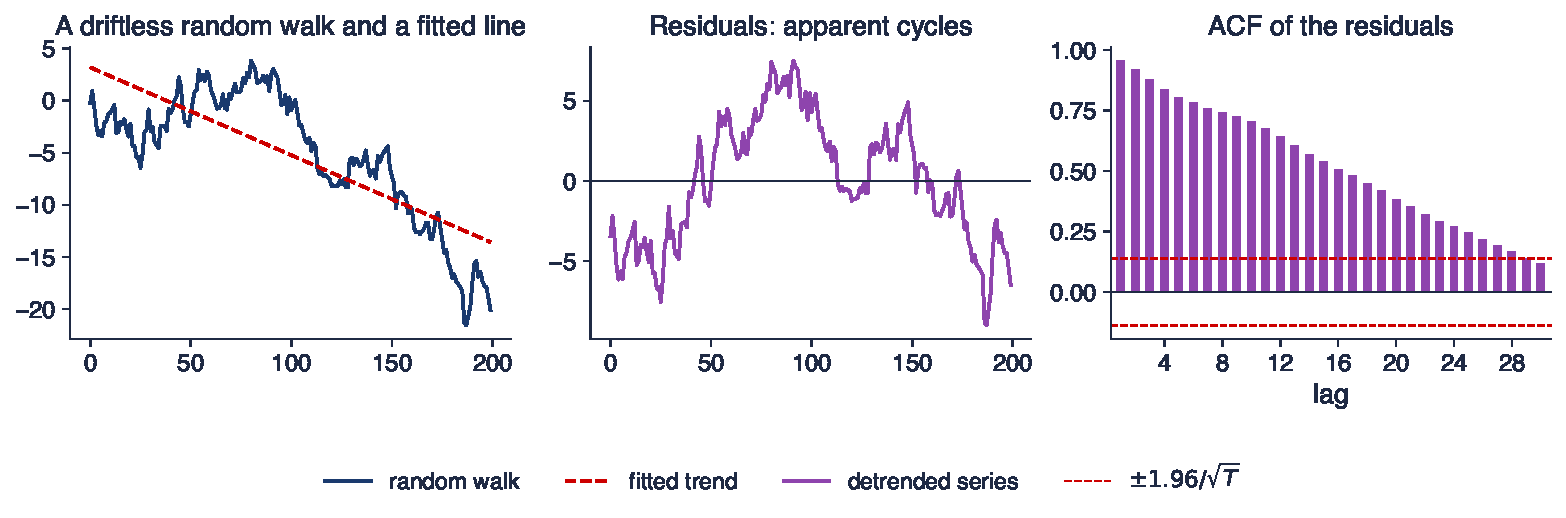
\includegraphics[width=0.97\textwidth,height=0.56\textheight,keepaspectratio]{tsa_ch3_detrend.pdf}
\end{center}
\vspace{-0.25cm}
\begin{itemize}
    \item Left: a driftless random walk ($T = 200$) and the OLS line $\hat a + \hat b t$; centre: the residuals; right: their ACF
\end{itemize}
\quantlet{TSA\_ch3\_trends}{\qlurl{TSA_ch3_trends}}
\end{frame}

\begin{frame}{Interpreting the detrended random walk}
\itemsize{\small}
\begin{itemize}
    \item The line fits: $R^2 = 0.61$, $t = \ensuremath{-}17.7$ for the slope, although the true slope is 0
    \begin{itemize}
        \item over 2\,000 random walks: $|t| > 1.96$ in 90\% of cases, median $R^2 = 0.44$
    \end{itemize}
    \item The residuals look like long cycles: $\hat\rho(1) = 0.96$ and a slow decay
    \begin{itemize}
        \item \refNK: detrending a DS series creates \textbf{spurious cycles}; a business cycle may be an artefact of the method
    \end{itemize}
    \item The reverse error (differencing a TS series) is over-differencing (\tsachlink{https://danpele.github.io/Time-Series-Analysis/EN/Courses/chapter1_stochastic_processes_stationarity.pdf}{Chapter 1} and Section 6)
\end{itemize}
\end{frame}

\begin{frame}{Recap: Deterministic and stochastic trends}
\itemsize{\small}
\begin{itemize}
    \item TS: $y_t = \alpha + \beta t + u_t$, shocks fade; DS: $\Delta y_t = \beta + u_t$, shocks are permanent
    \item $I(d)$: stationary after $d$ differences; a unit root in $\phi(z)$ means $I(1)$
    \item The wrong treatment creates artefacts: spurious cycles (detrending a DS series) or over-differencing (differencing a TS series)
\end{itemize}
\end{frame}


%=============================================================================
\section{Spurious regression}
%=============================================================================

\begin{frame}{1926: nonsense correlations}
\itemsize{\small}
\begin{itemize}
    \item \refYule\ asked: \textit{Why do we sometimes get nonsense-correlations between time-series?}
    \begin{itemize}
        \item his example: in England and Wales, 1866--1911, the share of Church of England marriages and the mortality rate had a correlation of about 0.95
        \item no causal link: both series simply declined over the period
    \end{itemize}
    \item His explanation: for series that wander like sums of random terms, the sample correlation does not settle near 0
    \begin{itemize}
        \item large values occur often by chance; the usual standard error does not apply
    \end{itemize}
    \item Fifty years later, the same problem reappeared in econometric models estimated on levels
\end{itemize}
\end{frame}

\begin{frame}{1974: Granger and Newbold}
\itemsize{\small}
\begin{columns}[T]
\begin{column}{0.30\textwidth}
\centering

\includegraphics[height=0.42\textheight]{ch3_clive_granger_2008.jpg}\\[1mm]
\imgcap{Clive Granger (1934--2009), Nobel Prize in Economics 2003}
\imgcredit{https://commons.wikimedia.org/wiki/File:Clive_Granger_by_Olaf_Storbeck_(3x4_cropped).jpg}{Photo: Olaf Storbeck (2008); CC BY-SA 2.0; Wikimedia Commons}
\end{column}
\begin{column}{0.66\textwidth}
\begin{itemize}
    \item \refGN: regress one random walk on another, \textbf{independent} random walk
    \begin{itemize}
        \item $y_t = a + b x_t + e_t$ with $y_t$, $x_t$ independent $I(1)$ series
        \item the $t$-test of $b = 0$ rejects far too often; $R^2$ is high; the Durbin--Watson statistic is close to 0
    \end{itemize}
    \item Their rule of thumb: be suspicious when $R^2 > \mathrm{DW}$
    \begin{itemize}
        \item DW (Durbin--Watson) $\approx 2(1 - \hat\rho_1)$ of the residuals: near 0 means $I(1)$-like residuals
    \end{itemize}
    \item Granger and Newbold were then at the University of Nottingham; Granger later received the Nobel Prize for cointegration (\tsachlink{https://danpele.github.io/Time-Series-Analysis/EN/Courses/chapter7_cointegration_vecm.pdf}{Chapter 7})
\end{itemize}
\end{column}
\end{columns}
\end{frame}

\begin{frame}{Spurious regression by simulation}
\itemsize{\footnotesize}
\begin{center}
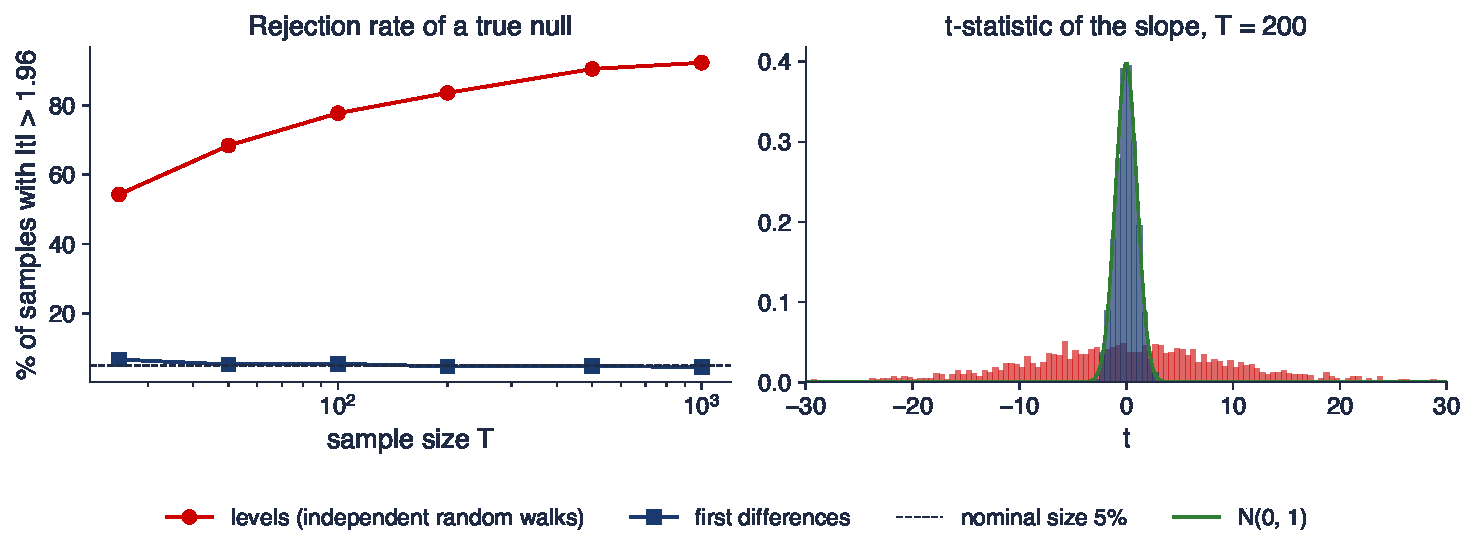
\includegraphics[width=0.97\textwidth,height=0.55\textheight,keepaspectratio]{tsa_ch3_spurious_mc.pdf}
\end{center}
\vspace{-0.25cm}
\begin{itemize}
    \item 2\,000 pairs of independent Gaussian random walks for each $T$; OLS of $y$ on a constant and $x$, in levels and in first differences
    \item Left: share of samples with $|t| > 1.96$; right: the distribution of $t$ for $T = 200$
\end{itemize}
\quantlet{TSA\_ch3\_spurious\_regression}{\qlurl{TSA_ch3_spurious_regression}}
\end{frame}

\begin{frame}{Interpreting the simulation}
\itemsize{\small}
\begin{itemize}
    \item Levels: a true null $b = 0$ is rejected in 68\% of samples with $T = 50$ and in 92\% with $T = 1000$
    \begin{itemize}
        \item more data makes it worse: the median $|t|$ grows from 3.2 ($T = 50$) to 14.2 ($T = 1000$)
        \item median $R^2$ about 0.17 for every $T$; median DW 0.08 at $T = 200$
    \end{itemize}
    \item Differences: 4.7\% at $T = 200$, close to the nominal 5\%
    \begin{itemize}
        \item the $t$-test works again because $\Delta y_t$ and $\Delta x_t$ are stationary
    \end{itemize}
\end{itemize}
\end{frame}

\begin{frame}{Why the $t$-test fails}
\itemsize{\small}
\begin{itemize}
    \item Under $b = 0$ the error $e_t = y_t - a$ is itself a random walk: the OLS assumptions (stationary, uncorrelated errors) fail
    \begin{itemize}
        \item the usual standard error is far too small
    \end{itemize}
    \item \refPhillips\ derived the large-sample behaviour
    \begin{itemize}
        \item $\hat b$ does not converge to 0: it converges to a random variable
        \item $t_{\hat b}$ grows like $\sqrt{T}$, so the rejection rate tends to 100\%
        \item $R^2$ has a non-degenerate limit distribution; $\mathrm{DW} \to 0$
    \end{itemize}
    \item Exception: if $y_t - b x_t$ is stationary for some $b$, the series are \textbf{cointegrated} and the levels regression is meaningful \refEG\ (\tsachlink{https://danpele.github.io/Time-Series-Analysis/EN/Courses/chapter7_cointegration_vecm.pdf}{Chapter 7})
\end{itemize}
\end{frame}

\begin{frame}{A spurious regression on real data}
\itemsize{\footnotesize}
\begin{center}
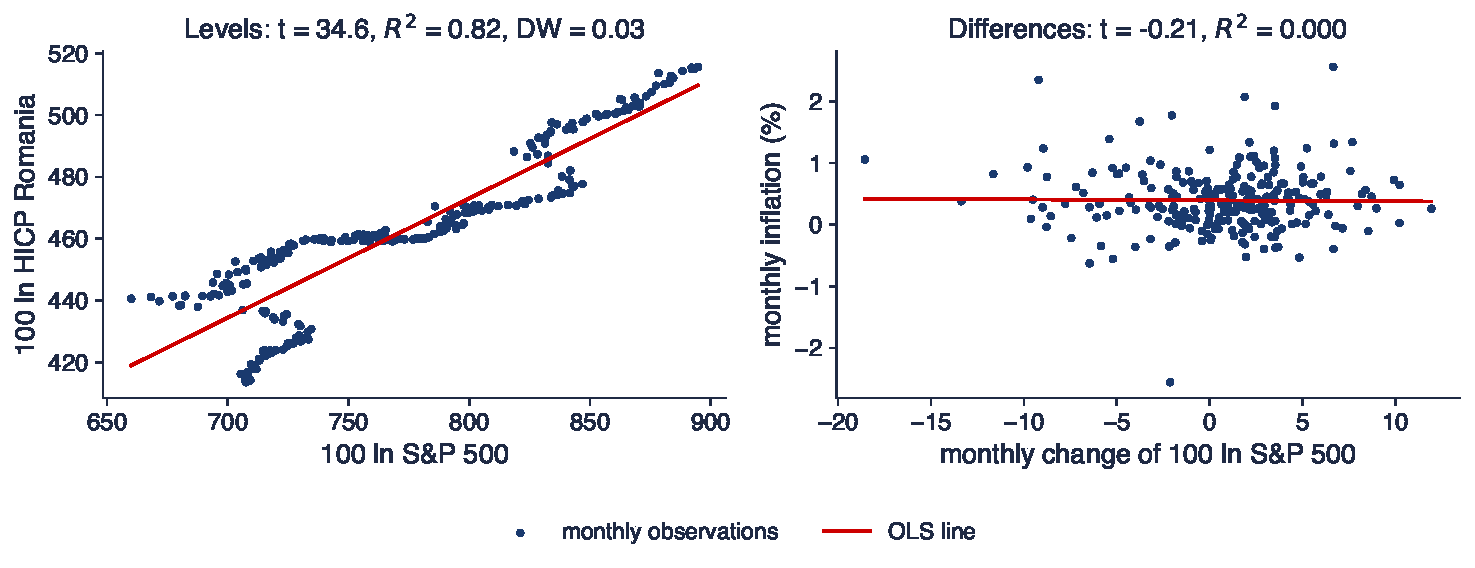
\includegraphics[width=0.97\textwidth,height=0.55\textheight,keepaspectratio]{tsa_ch3_spurious_real.pdf}
\end{center}
\vspace{-0.25cm}
\begin{itemize}
    \item Romanian HICP (Eurostat) against the S\&P 500 (month-end close), 260 months since January 2005, both as $100\ln$
    \item Left: levels; right: monthly changes
\end{itemize}
\quantlet{TSA\_ch3\_spurious\_regression}{\qlurl{TSA_ch3_spurious_regression}}
\end{frame}

\begin{frame}{Interpreting the HICP regression}
\itemsize{\small}
\begin{itemize}
    \item Levels: slope 0.39, $t = 34.6$, $R^2 = 0.82$, $\mathrm{DW} = 0.03$
    \begin{itemize}
        \item ``US stocks explain Romanian consumer prices'': $R^2 > \mathrm{DW}$, a textbook spurious regression
    \end{itemize}
    \item Differences: $t = \ensuremath{-}0.21$ (p = 0.83), $R^2 = 0.0002$
    \begin{itemize}
        \item monthly inflation and monthly stock returns are unrelated
    \end{itemize}
    \item Both levels contain a trend; the regression only says that both went up
\end{itemize}
\end{frame}

\begin{frame}{Recap: Spurious regression}
\itemsize{\small}
\begin{itemize}
    \item Regressing one $I(1)$ series on an unrelated $I(1)$ series gives large $t$, high $R^2$ and DW near 0
    \item More observations do not help: $t$ grows like $\sqrt{T}$
    \item Remedies: test the order of integration first; regress differences; or test for cointegration (\tsachlink{https://danpele.github.io/Time-Series-Analysis/EN/Courses/chapter7_cointegration_vecm.pdf}{Chapter 7})
\end{itemize}
\end{frame}


%=============================================================================
\section{The Dickey--Fuller test}
%=============================================================================

\begin{frame}{Testing $\phi = 1$}
\itemsize{\small}
\begin{itemize}
    \item AR(1): $y_t = \phi y_{t-1} + \varepsilon_t$; subtract $y_{t-1}$: $\Delta y_t = \gamma y_{t-1} + \varepsilon_t$, with $\gamma = \phi - 1$
    \begin{itemize}
        \item $H_0$: $\gamma = 0$ (unit root, $I(1)$); $H_1$: $\gamma < 0$ (stationary); a one-sided, left-tail test
        \item statistic: $\tau = \hat\gamma/\mathrm{SE}(\hat\gamma)$, the usual OLS $t$-ratio; $\mathrm{SE}$: the standard error; a very negative $\tau$ speaks against the unit root
    \end{itemize}
    \item Under $H_0$, $\tau$ is \textbf{not} Student or Normal \refDF
    \begin{itemize}
        \item $y_{t-1}$ is a random walk, so the regressor is not stationary; $\hat\phi$ converges at rate $T$, not $\sqrt{T}$ (\textbf{superconsistency})
        \item the limit of $\tau$ is a functional of Brownian motion, skewed to the left \refHamilton, Ch.~17
        \item critical values come from simulation: \refFuller; today from response surfaces \refMacKinnonb
    \end{itemize}
\end{itemize}
\end{frame}

\begin{frame}{Iowa State: where the test was born}
\itemsize{\small}
\begin{columns}[T]
\begin{column}{0.48\textwidth}
\centering

\includegraphics[height=0.44\textheight]{ch3_snedecor_hall_2023.jpg}\\[1mm]
\imgcap{Snedecor Hall, Iowa State University: the department of statistics and its Statistical Laboratory (1933)}
\imgcredit{https://commons.wikimedia.org/wiki/File:Snedecor_Hall,_Iowa_State_University.tif}{Photo: Maitra (2023); CC BY-SA 4.0; Wikimedia Commons}
\end{column}
\begin{column}{0.48\textwidth}
\begin{itemize}
    \item \textbf{Wayne A. Fuller}: statistician at Iowa State, author of \textit{Introduction to Statistical Time Series} \refFuller
    \item \textbf{David A. Dickey}: his doctoral student at Iowa State (1976), later at North Carolina State University
    \item \refDF: the distribution of $\hat\phi$ and $\tau$ under a unit root; \refDFb: joint tests of the unit root and the deterministic terms
    \item \refSD: the augmented test for ARMA errors (this section)
\end{itemize}
\end{column}
\end{columns}
\end{frame}

\begin{frame}{Three Dickey--Fuller regressions}
\itemsize{\small}
\begin{itemize}
    \item \textbf{No constant}: $\Delta y_t = \gamma y_{t-1} + \varepsilon_t$
    \begin{itemize}
        \item $H_1$: stationary with mean 0; rarely realistic
    \end{itemize}
    \item \textbf{Constant}: $\Delta y_t = c + \gamma y_{t-1} + \varepsilon_t$
    \begin{itemize}
        \item $H_0$: random walk (with drift if $c \ne 0$); $H_1$: stationary around a non-zero mean
        \item for series without a trend: interest rates, inflation, exchange rates, returns
    \end{itemize}
    \item \textbf{Constant and trend}: $\Delta y_t = c + bt + \gamma y_{t-1} + \varepsilon_t$
    \begin{itemize}
        \item $c$: the constant; $bt$: a linear trend with slope $b$
        \item $H_0$: random walk with drift; $H_1$: trend-stationary: exactly the TS against DS question of Section 1
        \item for trending series: log GDP, log prices, log price indices
    \end{itemize}
    \item Each case has its own distribution of $\tau$ and its own critical values
\end{itemize}
\end{frame}

\begin{frame}{The Dickey--Fuller distributions}
\itemsize{\footnotesize}
\begin{center}
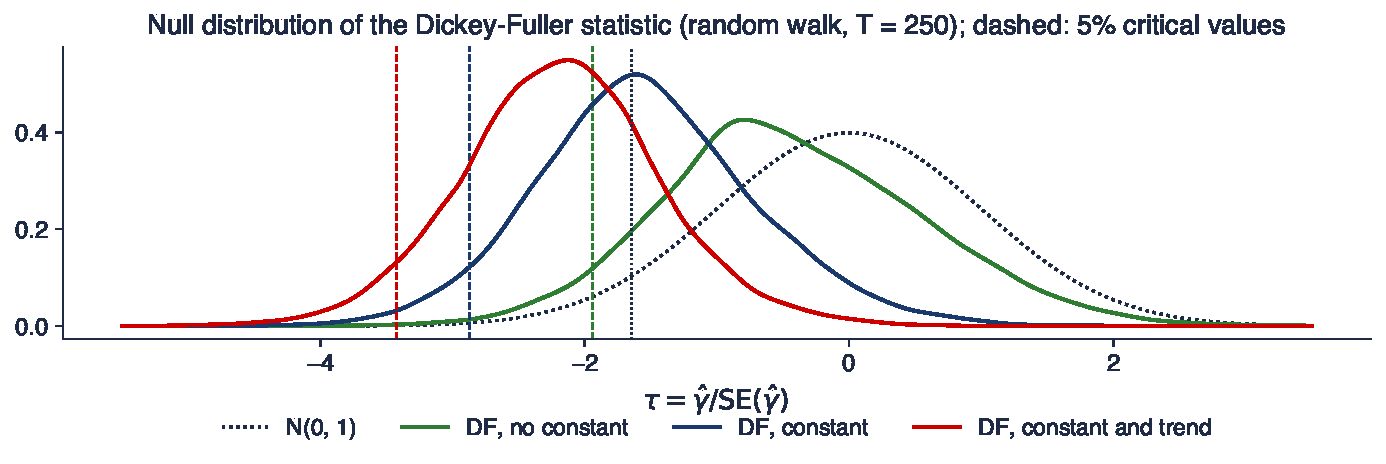
\includegraphics[width=0.97\textwidth,height=0.56\textheight,keepaspectratio]{tsa_ch3_df_dist.pdf}
\end{center}
\vspace{-0.25cm}
\begin{itemize}
    \item 20\,000 random walks with $T = 250$: the density of $\tau$ in the three regressions, against $N(0, 1)$; dashed lines: 5\% critical values \refMacKinnonb
\end{itemize}
\quantlet{TSA\_ch3\_dickey\_fuller}{\qlurl{TSA_ch3_dickey_fuller}}
\end{frame}

\begin{frame}{Interpreting the three distributions}
\itemsize{\small}
\begin{itemize}
    \item All three lie to the left of $N(0, 1)$; the more deterministic terms, the further left
    \begin{itemize}
        \item simulated 5\% quantiles: $\ensuremath{-}1.95$ (no constant), $\ensuremath{-}2.86$ (constant) and $\ensuremath{-}3.42$ (constant and trend); tabulated: $\ensuremath{-}1.94$, $\ensuremath{-}2.87$ and $\ensuremath{-}3.43$
    \end{itemize}
    \item With the Normal critical value $-1.645$, a true unit root is ``rejected'' in 46\% of samples (constant) and 77\% (constant and trend)
    \begin{itemize}
        \item the wrong table turns random walks into ``stationary'' series
    \end{itemize}
\end{itemize}
\end{frame}

\begin{frame}{Critical values of the Dickey--Fuller test}
\itemsize{\small}
\begin{center}
\scriptsize
\begin{tabular}{lccc|ccc|ccc}
\toprule
& \multicolumn{3}{c|}{\textbf{no constant}} & \multicolumn{3}{c|}{\textbf{constant}} & \multicolumn{3}{c}{\textbf{constant and trend}} \\ $T$ & 1\% & 5\% & 10\% & 1\% & 5\% & 10\% & 1\% & 5\% & 10\% \\
\midrule
50 & $\ensuremath{-}2.61$ & $\ensuremath{-}1.95$ & $\ensuremath{-}1.61$ & $\ensuremath{-}3.57$ & $\ensuremath{-}2.92$ & $\ensuremath{-}2.60$ & $\ensuremath{-}4.15$ & $\ensuremath{-}3.50$ & $\ensuremath{-}3.18$ \\
100 & $\ensuremath{-}2.59$ & $\ensuremath{-}1.94$ & $\ensuremath{-}1.61$ & $\ensuremath{-}3.50$ & $\ensuremath{-}2.89$ & $\ensuremath{-}2.58$ & $\ensuremath{-}4.05$ & $\ensuremath{-}3.46$ & $\ensuremath{-}3.15$ \\
250 & $\ensuremath{-}2.57$ & $\ensuremath{-}1.94$ & $\ensuremath{-}1.62$ & $\ensuremath{-}3.46$ & $\ensuremath{-}2.87$ & $\ensuremath{-}2.57$ & $\ensuremath{-}4.00$ & $\ensuremath{-}3.43$ & $\ensuremath{-}3.14$ \\
$\infty$ & $\ensuremath{-}2.57$ & $\ensuremath{-}1.94$ & $\ensuremath{-}1.62$ & $\ensuremath{-}3.43$ & $\ensuremath{-}2.86$ & $\ensuremath{-}2.57$ & $\ensuremath{-}3.96$ & $\ensuremath{-}3.41$ & $\ensuremath{-}3.13$ \\
\bottomrule
\end{tabular}
\end{center}
\begin{itemize}
    \item Source: the response surfaces of \refMacKinnonb, as used by \texttt{statsmodels}; p-values from \refMacKinnon
    \item Decision: reject the unit root at 5\% if $\tau$ is \textbf{below} (more negative than) the 5\% value
    \item The values depend only weakly on $T$; they apply unchanged to the ADF test
\end{itemize}
\end{frame}

\begin{frame}{Worked example: Romanian real GDP}
\itemsize{\small}
\begin{itemize}
    \item $y_t = 100\ln$ real GDP, 2000Q1--2026Q2; regression with constant and trend, no lags ($T = 105$ differences)
    \begin{itemize}
        \item OLS: $\hat\gamma = \ensuremath{-}0.0961$, $\mathrm{SE}(\hat\gamma) = 0.0416$, so $\hat\phi = 1 + \hat\gamma = 0.904$
    \end{itemize}
    \item $\tau = \ensuremath{-}0.0961/0.0416 = \ensuremath{-}2.31$; 5\% critical value with constant and trend: $\ensuremath{-}3.45$
    \begin{itemize}
        \item $\ensuremath{-}2.31 > \ensuremath{-}3.45$: do not reject the unit root (p = 0.43)
        \item with the Normal value $-1.645$ we would have rejected it: the wrong table gives the wrong answer
    \end{itemize}
    \item Reading: ``not rejected'' is not ``proved''
    \begin{itemize}
        \item if $\phi = 0.904$ were true, a shock would halve in $\ln 0.5/\ln 0.904 \approx 6.9$ quarters; with 106 observations the test can hardly tell this from $\phi = 1$
    \end{itemize}
\end{itemize}
\end{frame}

\begin{frame}{The augmented Dickey--Fuller test}
\itemsize{\small}
\begin{itemize}
    \item If $\Delta y_t$ is autocorrelated, $\varepsilon_t$ in the DF regression is not white noise and the size of the test is wrong
    \begin{itemize}
        \item the remedy: add lagged differences
    \end{itemize}
    \item \textbf{ADF} (augmented Dickey--Fuller) regression:
    \begin{itemize}
        \item $\Delta y_t = c + bt + \gamma y_{t-1} + \sum_{j=1}^{k} \delta_j \Delta y_{t-j} + \varepsilon_t$; same $\tau$, same critical values
        \item $\delta_j$: the coefficients of the past differences; $k$: the number of lagged differences
        \item an AR($p$) in levels becomes exactly this regression with $k = p - 1$ and $\gamma = -\phi(1)$
    \end{itemize}
    \item \refSD: with ARMA errors the test stays valid if $k$ grows slowly with $T$
    \begin{itemize}
        \item the lags approximate the MA part by a long AR
    \end{itemize}
    \item The ADF test is the default unit-root test in software: \texttt{adfuller} in \texttt{statsmodels}
\end{itemize}
\end{frame}

\begin{frame}{Choosing the number of lags $k$}
\itemsize{\small}
\begin{itemize}
    \item Maximum: $k_{\max} = 12\,(T/100)^{1/4}$ \refSchwert; for $T = 105$, $k_{\max} = 13$
    \begin{itemize}
        \item then choose $k \le k_{\max}$ by an information criterion, AIC or BIC (\tsachlink{https://danpele.github.io/Time-Series-Analysis/EN/Courses/chapter2_arma_models.pdf}{Chapter 2}), on the same sample for every $k$
    \end{itemize}
    \item Too few lags: autocorrelated errors, wrong size (with a negative MA part, far too many rejections)
    \begin{itemize}
        \item too many lags: lower power
    \end{itemize}
    \item \refNgP: a modified AIC (MAIC) gives a better size; GLS detrending \refERS\ gives more power
    \begin{itemize}
        \item MAIC: modified Akaike information criterion; GLS: generalised least squares; both appear in the DF-GLS test
    \end{itemize}
    \item Check the result: Ljung--Box on the ADF residuals \refLB; report $k$ together with $\tau$
\end{itemize}
\end{frame}

\begin{frame}{Size and power of the Dickey--Fuller test}
\itemsize{\footnotesize}
\begin{center}
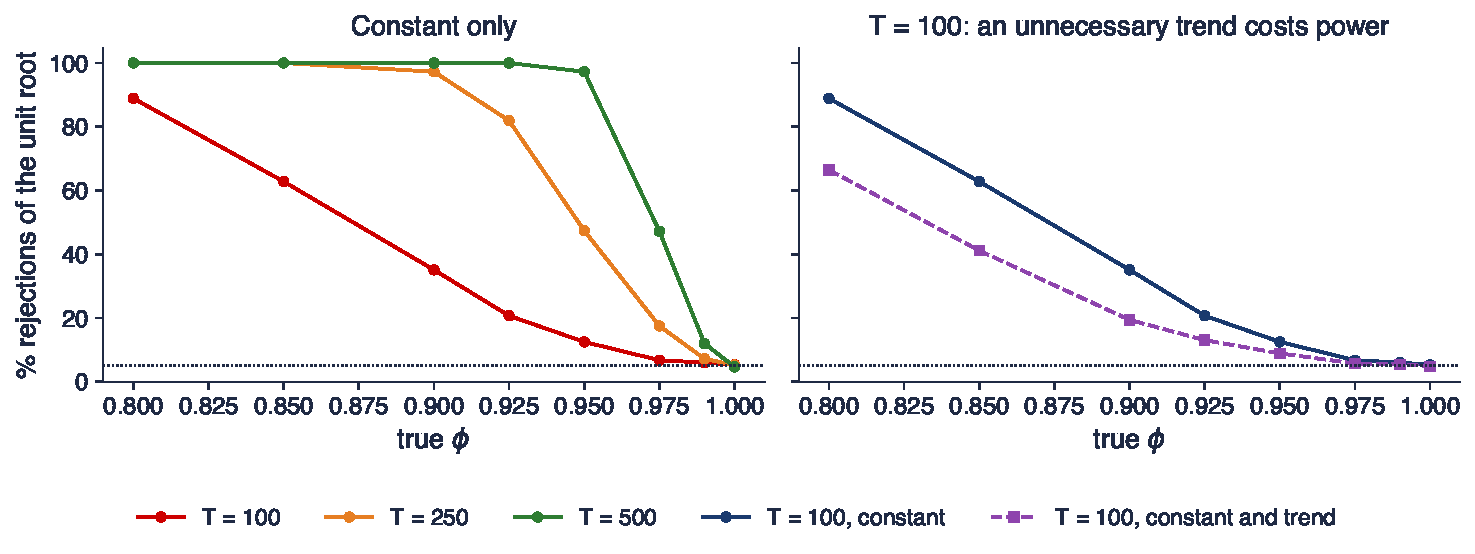
\includegraphics[width=0.97\textwidth,height=0.55\textheight,keepaspectratio]{tsa_ch3_adf_power.pdf}
\end{center}
\vspace{-0.25cm}
\begin{itemize}
    \item 2\,000 AR(1) paths $y_t = \phi y_{t-1} + \varepsilon_t$ for each $\phi$; share of rejections at 5\%; at $\phi = 1$ this is the size
\end{itemize}
\quantlet{TSA\_ch3\_dickey\_fuller}{\qlurl{TSA_ch3_dickey_fuller}}
\end{frame}

\begin{frame}{Interpreting the power curves}
\itemsize{\small}
\begin{itemize}
    \item Size: 5\%, 5\% and 5\% at $\phi = 1$: the test holds its 5\% level
    \item Power at $\phi = 0.95$: 12\% with $T = 100$, 47\% with $T = 250$, 97\% with $T = 500$
    \begin{itemize}
        \item a quarterly series of 25 years ($T = 100$) almost never distinguishes $\phi = 0.95$ from a unit root
        \item what matters is the time span, not the frequency: daily data over two years do not help
    \end{itemize}
    \item An unnecessary trend costs power: at $T = 100$ and $\phi = 0.9$, 35\% with a constant, 19\% with constant and trend
\end{itemize}
\end{frame}

\begin{frame}{Choosing the deterministic terms}
\itemsize{\small}
\begin{itemize}
    \item The alternative must be a plausible description of the data
    \begin{itemize}
        \item trending series (log GDP, log prices): constant and trend
        \item series that fluctuate around a level (interest rates, inflation, exchange rates, returns): constant
    \end{itemize}
    \item Omitting a needed trend: a TS series looks like a unit root; the test almost never rejects
    \begin{itemize}
        \item adding an unneeded trend: lower power (previous chart)
    \end{itemize}
    \item Look at the plot first, then choose; \refDFb\ give joint $F$-type tests of the unit root and the trend
\end{itemize}
\end{frame}

\begin{frame}{How many differences: $I(1)$ or $I(2)$?}
\itemsize{\small}
\begin{itemize}
    \item \refDP: test from the highest plausible order downwards
    \begin{itemize}
        \item step 1: ADF on $\Delta y_t$; if it does not reject, $y_t$ may be $I(2)$
        \item step 2: if it rejects, ADF on $y_t$; reject: $I(0)$; do not reject: $I(1)$
    \end{itemize}
    \item Why downwards: if $y_t \sim I(2)$, the test on $y_t$ assumes at most one unit root and is not valid
    \item Example: Romanian consumer prices since 2005 (the table in Section 4)
    \begin{itemize}
        \item $\ln P$: unit root; inflation $\pi$: ADF p = 0.32, KPSS 0.404; change of inflation: clearly stationary
        \item so $\ln P$ is $I(1)$ or $I(2)$, depending on how persistent inflation is: Section 7 returns to this
    \end{itemize}
\end{itemize}
\end{frame}

\begin{frame}{Recap: The Dickey--Fuller test}
\itemsize{\small}
\begin{itemize}
    \item $\Delta y_t = c + bt + \gamma y_{t-1} + \sum_j\delta_j\Delta y_{t-j} + \varepsilon_t$; $H_0$: $\gamma = 0$; $\tau$ against Dickey--Fuller critical values
    \item Deterministic terms follow the plot; lags by AIC or BIC up to $12(T/100)^{1/4}$
    \item Low power near $\phi = 1$: not rejecting is weak evidence for a unit root
    \item Order of integration: test from the top ($\Delta y_t$ first)
\end{itemize}
\end{frame}


%=============================================================================
\section{Phillips--Perron, KPSS and their joint use}
%=============================================================================

\begin{frame}{The Phillips--Perron test}
\itemsize{\small}
\begin{itemize}
    \item \refPP: keep the simple DF regression (no lagged differences) and correct $\tau$ instead
    \begin{itemize}
        \item $Z_\tau = \sqrt{\hat\gamma_0/\hat\lambda^2}\;\tau - \dfrac{(\hat\lambda^2 - \hat\gamma_0)\,T\,\mathrm{SE}(\hat\gamma)}{2\hat\lambda\,s}$
        \item $\hat\gamma_0$: variance of the residuals; $s^2$: their OLS variance; $\hat\lambda^2$: their \textbf{long-run variance}
    \end{itemize}
    \item Long-run variance (Newey--West, Bartlett weights): $\hat\lambda^2 = \hat\gamma_0 + 2\sum_{j=1}^{L}(1 - \frac{j}{L+1})\hat\gamma_j$
    \begin{itemize}
        \item $\hat\gamma_j$: autocovariances of the residuals; $L$: the number of autocovariances included (the bandwidth)
        \item if the residuals are white noise, $\hat\lambda^2 = \hat\gamma_0$ and $Z_\tau = \tau$: the correction only matters when they are autocorrelated
    \end{itemize}
    \item Same $H_0$ and the same critical values as ADF; robust to heteroskedasticity; no lag choice, but a bandwidth $L$
    \begin{itemize}
        \item weak point: large size distortions with a negative MA component \refSchwert
    \end{itemize}
\end{itemize}
\end{frame}

\begin{frame}{The KPSS test: stationarity as the null}
\itemsize{\small}
\begin{itemize}
    \item \refKPSS\ (KPSS: Kwiatkowski--Phillips--Schmidt--Shin): $y_t = \xi t + r_t + \varepsilon_t$, $r_t = r_{t-1} + u_t$, $u_t \sim \mathrm{WN}(0, \sigma_u^2)$
    \begin{itemize}
        \item $\xi t$: a deterministic trend; $r_t$: a random walk, the moving level; $\varepsilon_t$: stationary noise
        \item $H_0$: $\sigma_u^2 = 0$ (the random walk is a constant: $y_t$ stationary around a level or a trend); $H_1$: $\sigma_u^2 > 0$, a unit root
    \end{itemize}
    \item Statistic: regress $y_t$ on a constant (and a trend); residuals $e_t$; partial sums $S_t = e_1 + \dots + e_t$
    \begin{itemize}
        \item $\eta = \dfrac{1}{T^2\hat\lambda^2}\sum_{t=1}^{T} S_t^2$, with $\hat\lambda^2$ the long-run variance of $e_t$
        \item reject stationarity for \textbf{large} $\eta$: 5\% critical values 0.463 (level) and 0.146 (trend); 1\%: 0.739 and 0.216
    \end{itemize}
    \item A test of stationarity, not of a unit root: it reverses the burden of proof
\end{itemize}
\end{frame}

\begin{frame}{KPSS: why partial sums}
\itemsize{\footnotesize}
\begin{center}
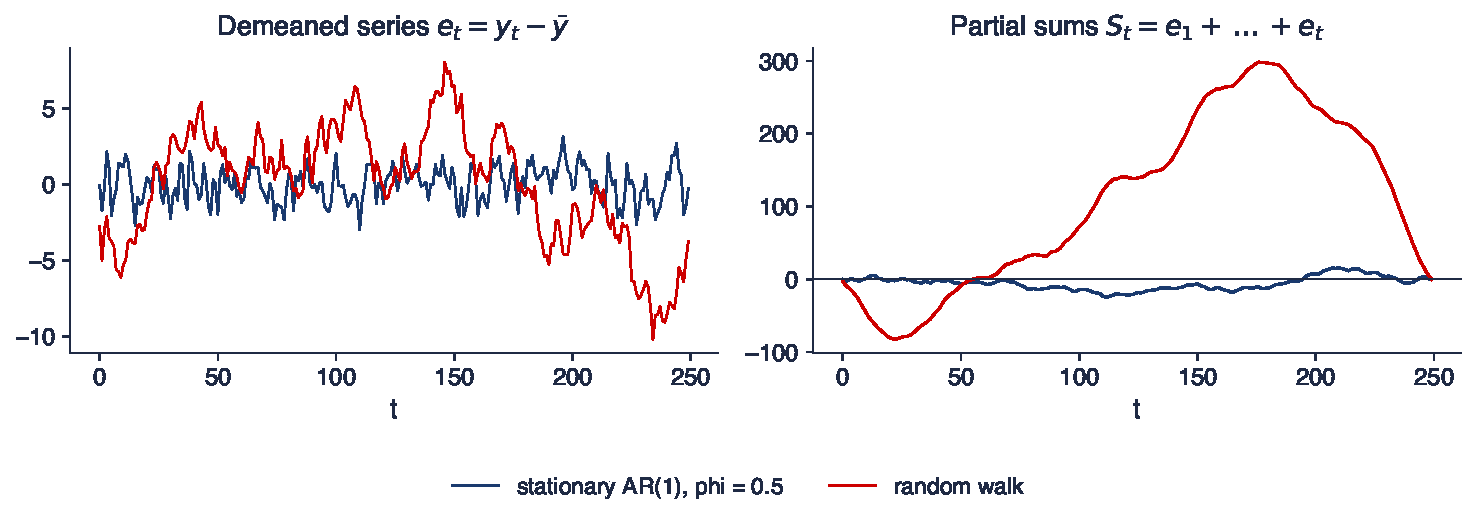
\includegraphics[width=0.97\textwidth,height=0.52\textheight,keepaspectratio]{tsa_ch3_kpss_sums.pdf}
\end{center}
\vspace{-0.25cm}
\begin{itemize}
    \item A stationary AR(1) ($\phi = 0.5$) and a random walk, $T = 250$: the demeaned series and their partial sums $S_t$
    \item KPSS (level): 0.16 for the AR(1), 0.73 for the random walk; 5\% critical value 0.463
\end{itemize}
\quantlet{TSA\_ch3\_unit\_root\_tests}{\qlurl{TSA_ch3_unit_root_tests}}
\end{frame}

\begin{frame}{Interpreting the partial sums}
\itemsize{\small}
\begin{itemize}
    \item Stationary series: deviations cancel out, $S_t$ stays close to 0
    \begin{itemize}
        \item $\sum S_t^2$ grows like $T^2$, so $\eta$ stays bounded
    \end{itemize}
    \item Random walk: long runs on one side of the mean, $S_t$ makes large excursions
    \begin{itemize}
        \item $\sum S_t^2$ grows like $T^4$: $\eta$ grows with $T$ and the test rejects
    \end{itemize}
    \item The same idea as the CUSUM charts of quality control: cumulated deviations reveal a drifting level
\end{itemize}
\end{frame}

\begin{frame}{ADF and KPSS together}
\itemsize{\small}
\begin{center}
\footnotesize
\begin{tabular}{lll}
\toprule
& \textbf{KPSS does not reject} & \textbf{KPSS rejects} \\
\midrule
\textbf{ADF rejects} & $I(0)$: both agree & conflict: break, long memory, outliers? \\
\textbf{ADF does not reject} & inconclusive: the data cannot decide & $I(1)$: both agree \\
\bottomrule
\end{tabular}
\end{center}
\begin{itemize}
    \item The two tests have opposite null hypotheses: agreement is stronger evidence than either test alone
    \item Inconclusive is common with short samples: low power on both sides
    \begin{itemize}
        \item then decide by the purpose: for forecasting, $d = 1$ is the cautious choice (wider intervals)
    \end{itemize}
    \item Conflict: look for breaks (Section 5) or fractional integration (\tsachlink{https://danpele.github.io/Time-Series-Analysis/EN/Courses/chapter8_long_memory_arfima.pdf}{Chapter 8})
\end{itemize}
\end{frame}

\begin{frame}{Unit-root tests on real series}
\itemsize{\scriptsize}
\begin{center}
\scriptsize
\begin{tabular}{llrrrrrl}
\toprule
\textbf{Series} & \textbf{det.} & $T$ & \textbf{ADF} (p) & $k$ & \textbf{PP} & \textbf{KPSS} & \textbf{ADF+KPSS} \\
\midrule
Romania, real GDP, $100\ln Y$ & c, t & 106 & $\ensuremath{-}2.31$ (0.428) & 0 & $\ensuremath{-}2.19$ & 0.198 & $I(1)$ \\
\quad its growth $\Delta$ & c & 105 & $\ensuremath{-}10.77$ ($<$\,0.001) & 0 & $\ensuremath{-}10.88$ & 0.263 & $I(0)$ \\
Romania, HICP, $100\ln P$ & c, t & 260 & $\ensuremath{-}0.96$ (0.949) & 6 & $\ensuremath{-}0.88$ & 0.314 & $I(1)$ \\
Romania, 12-month inflation $\pi$ & c & 260 & $\ensuremath{-}1.94$ (0.315) & 15 & $\ensuremath{-}2.31$ & 0.404 & inconclusive \\
\quad its change $\Delta\pi$ & c & 259 & $\ensuremath{-}4.83$ ($<$\,0.001) & 14 & $\ensuremath{-}11.31$ & 0.105 & $I(0)$ \\
US, real GDP, $100\ln Y$ & c, t & 318 & $\ensuremath{-}1.54$ (0.816) & 1 & $\ensuremath{-}1.20$ & 0.581 & $I(1)$ \\
\quad its growth $\Delta$ & c & 317 & $\ensuremath{-}15.51$ ($<$\,0.001) & 0 & $\ensuremath{-}15.44$ & 0.456 & $I(0)$ \\
EUR/RON, $100\ln S$ & c & 5\,353 & $\ensuremath{-}1.22$ (0.664) & 7 & $\ensuremath{-}1.15$ & 10.255 & $I(1)$ \\
\quad daily returns & c & 5\,352 & $\ensuremath{-}27.42$ ($<$\,0.001) & 6 & $\ensuremath{-}60.82$ & 0.055 & $I(0)$ \\
BET, $100\ln P$ & c, t & 6\,671 & $\ensuremath{-}1.90$ (0.653) & 19 & $\ensuremath{-}2.35$ & 1.143 & $I(1)$ \\
\quad daily returns & c & 6\,670 & $\ensuremath{-}16.50$ ($<$\,0.001) & 18 & $\ensuremath{-}74.55$ & 0.360 & $I(0)$ \\
S\&P 500, $100\ln P$ & c, t & 6\,715 & $\ensuremath{-}2.08$ (0.557) & 34 & $\ensuremath{-}2.36$ & 2.281 & $I(1)$ \\
\quad daily returns & c & 6\,714 & $\ensuremath{-}14.26$ ($<$\,0.001) & 35 & $\ensuremath{-}91.41$ & 0.449 & $I(0)$ \\
Nile, yearly flow & c & 100 & $\ensuremath{-}4.05$ (0.001) & 1 & $\ensuremath{-}6.38$ & 0.869 & conflict \\
\bottomrule
\end{tabular}
\end{center}
\begin{itemize}
    \item det.: deterministic terms (c: constant; t: trend); $k$: ADF lags (AIC); 5\% critical values: ADF and PP about $-2.86$ (c), $-3.41$ (c, t); KPSS 0.463 (c), 0.146 (c, t)
\end{itemize}\quantlet{TSA\_ch3\_unit\_root\_tests}{\qlurl{TSA_ch3_unit_root_tests}}
\end{frame}

\begin{frame}{Interpreting the unit-root table}
\itemsize{\small}
\begin{itemize}
    \item Log prices, the exchange rate, log GDP and log HICP: $I(1)$; their differences: $I(0)$
    \begin{itemize}
        \item Romanian GDP: ADF p = 0.43 and KPSS 0.198 $> 0.146$: a unit root, as \refNP\ found for the US
    \end{itemize}
    \item Romanian 12-month inflation: neither test rejects (KPSS 0.404 $< 0.463$): inconclusive
    \begin{itemize}
        \item a very persistent series, possibly with breaks; Sections 5 and 7
    \end{itemize}
    \item Nile: both reject: a conflict
    \begin{itemize}
        \item \tsachlink{https://danpele.github.io/Time-Series-Analysis/EN/Courses/chapter1_stochastic_processes_stationarity.pdf}{Chapter 1} showed a level shift in 1898: the next section explains the conflict
    \end{itemize}
    \item Daily returns: PP gives far more negative values than ADF (BET: $\ensuremath{-}74.6$ against $\ensuremath{-}16.5$), but both reject; the verdict is the same
\end{itemize}
\end{frame}

\begin{frame}{Recap: Phillips--Perron and KPSS}
\itemsize{\small}
\begin{itemize}
    \item PP: DF regression plus a long-run-variance correction; same $H_0$ and critical values as ADF
    \item KPSS: $H_0$ stationarity; large partial sums reject it
    \item Read ADF and KPSS together: agree, inconclusive, or conflict
\end{itemize}
\end{frame}


%=============================================================================
\section{Structural breaks}
%=============================================================================

\begin{frame}{Perron (1989): a break can look like a unit root}
\itemsize{\small}
\begin{itemize}
    \item \refPerron: a stationary series around a mean or a trend that \textbf{shifts once} looks persistent
    \begin{itemize}
        \item the DF regression explains the shift by $\hat\phi$ close to 1; the test loses power
    \end{itemize}
    \item He re-examined Nelson and Plosser with two known breaks: the 1929 crash (level) and the 1973 oil shock (slope)
    \begin{itemize}
        \item with dummy variables for the break, the unit root was rejected for most series
        \item reading: most shocks are transitory; only a few rare events are permanent
    \end{itemize}
    \item The critique: the break date was chosen after looking at the data
\end{itemize}
\end{frame}

\begin{frame}{A level shift misleads the ADF test}
\itemsize{\footnotesize}
\begin{center}
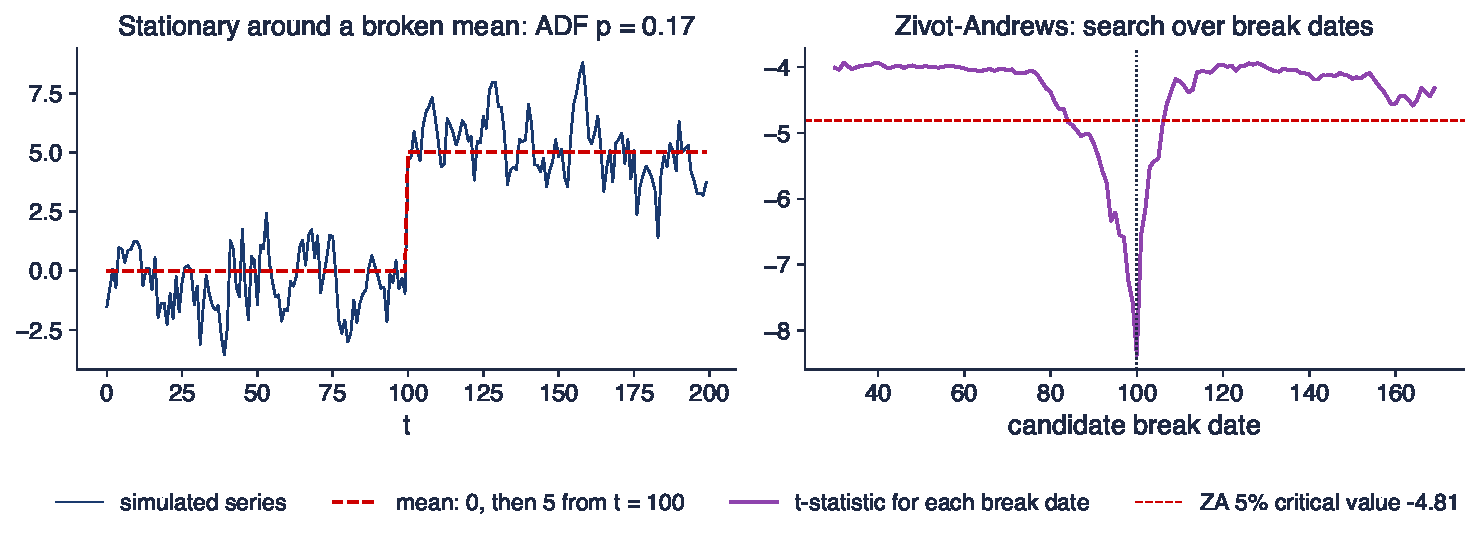
\includegraphics[width=0.97\textwidth,height=0.54\textheight,keepaspectratio]{tsa_ch3_breaks_sim.pdf}
\end{center}
\vspace{-0.25cm}
\begin{itemize}
    \item Left: AR(1) noise ($\phi = 0.6$) around a mean that jumps from 0 to 5 at $t = 100$; right: the $t$-statistic on $y_{t-1}$ for every candidate break date, with a level dummy
\end{itemize}
\quantlet{TSA\_ch3\_structural\_breaks}{\qlurl{TSA_ch3_structural_breaks}}
\end{frame}

\begin{frame}{Interpreting the simulated break}
\itemsize{\small}
\begin{itemize}
    \item ADF with a constant: p = 0.17: the stationary series ``has a unit root''
    \begin{itemize}
        \item over 2\,000 such series, the DF test rejects in 72\% of cases; without the break: 100\%
    \end{itemize}
    \item With the break modelled, the statistic falls to $\ensuremath{-}7.47$, far below the 5\% value $\ensuremath{-}4.81$
    \begin{itemize}
        \item the minimum is reached at the true date $t = 100$
    \end{itemize}
\end{itemize}
\end{frame}

\begin{frame}{Zivot and Andrews (1992): an unknown break date}
\itemsize{\small}
\begin{itemize}
    \item \refZA: let the data choose the break date $T_B$
    \begin{itemize}
        \item for each $T_B$ in the central 70\% of the sample, run the ADF regression with a break dummy:
        \item $\Delta y_t = c + \theta DU_t + bt + \gamma y_{t-1} + \sum_j\delta_j\Delta y_{t-j} + \varepsilon_t$, $DU_t = 1$ for $t > T_B$
        \item $DU_t$: a dummy variable, 0 before and 1 after the break; $\theta$: the size of the level shift
        \item the statistic is the \textbf{minimum} $t$-ratio of $\gamma$ over all dates
    \end{itemize}
    \item Three versions: break in the level, in the slope, in both
    \begin{itemize}
        \item critical values more negative than ADF: about $-4.81$ (level) and $-5.07$ (both) at 5\%
    \end{itemize}
    \item $H_0$: unit root without a break; $H_1$: stationary with one break
    \begin{itemize}
        \item several breaks: \refBaiP; a rejection does not prove that the break is the right story
    \end{itemize}
\end{itemize}
\end{frame}

\begin{frame}{Zivot--Andrews on two real series}
\itemsize{\footnotesize}
\begin{center}
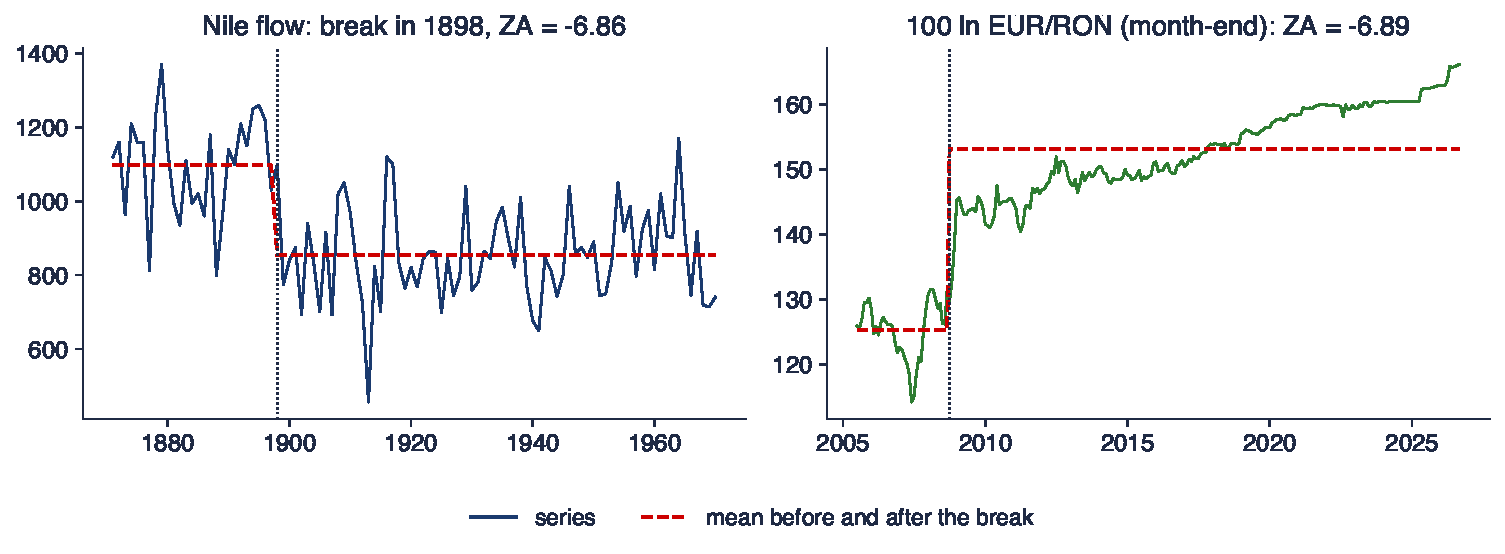
\includegraphics[width=0.97\textwidth,height=0.54\textheight,keepaspectratio]{tsa_ch3_breaks_real.pdf}
\end{center}
\vspace{-0.25cm}
\begin{itemize}
    \item Left: the Nile flow (statsmodels data set, 1871--1970); right: 100 ln EUR/RON, month-end BNR reference rate
    \item Dotted line: the break date chosen by the test (break in the level)
\end{itemize}
\quantlet{TSA\_ch3\_structural\_breaks}{\qlurl{TSA_ch3_structural_breaks}}
\end{frame}

\begin{frame}{Interpreting the two breaks}
\itemsize{\small}
\begin{itemize}
    \item Nile: ZA = $\ensuremath{-}6.86$, break in 1898, the mean falls from 1098 to 853
    \begin{itemize}
        \item the date matches the history: the first Aswan dam (built 1898--1902) and a drier climate; the ADF--KPSS conflict is explained
    \end{itemize}
    \item EUR/RON (month-end): ADF p = 0.55, but ZA = $\ensuremath{-}6.89$, break in October 2008: the 2008 depreciation (mean 3.50 lei before, 4.62 after)
    \begin{itemize}
        \item a managed exchange rate: long calm periods and rare adjustments, not a pure random walk
        \item but after 2008 the rate still drifts up: ``stationary around one break'' is also a simplification
    \end{itemize}
\end{itemize}
\end{frame}

\begin{frame}{Recap: Structural breaks}
\itemsize{\small}
\begin{itemize}
    \item A one-time shift in the mean or trend biases unit-root tests towards non-rejection
    \item Zivot--Andrews searches the break date; its critical values are more negative
    \item Unit root or break: check the dates against known events
\end{itemize}
\end{frame}


%=============================================================================
\section{ARIMA$(p,d,q)$ models}
%=============================================================================

\begin{frame}{The ARIMA model}
\itemsize{\small}
\begin{itemize}
    \item \textbf{Definition}: $y_t \sim$ ARIMA$(p,d,q)$ (autoregressive integrated moving average) if $\Delta^d y_t$ is a stationary, invertible ARMA$(p,q)$:
    \begin{itemize}
        \item $\phi(L)\,(1 - L)^d\,y_t = c + \theta(L)\,\varepsilon_t$, $\varepsilon_t \sim \mathrm{WN}(0, \sigma^2)$
        \item $p$: AR order; $d$: number of differences (unit roots); $q$: MA order; $\phi(L)$, $\theta(L)$ as in \tsachlink{https://danpele.github.io/Time-Series-Analysis/EN/Courses/chapter2_arma_models.pdf}{Chapter 2}
    \end{itemize}
    \item The AR polynomial of the levels is $\phi(z)(1 - z)^d$: $d$ roots exactly on the unit circle
    \begin{itemize}
        \item ``integrated'': $y_t$ is a $d$-fold cumulative sum of an ARMA process
    \end{itemize}
    \item \refBJ\ made the model popular; in practice $d \le 2$, and $d = 1$ most often
\end{itemize}
\end{frame}

\begin{frame}{Special cases and the constant}
\itemsize{\small}
\begin{center}
\scriptsize
\begin{tabular}{ll}
\toprule
\textbf{Model} & \textbf{Equation and meaning} \\
\midrule
ARIMA(0,1,0) & $\Delta y_t = c + \varepsilon_t$: random walk (with drift $c$) \\
ARIMA(1,1,0) & $\Delta y_t = c + \phi\Delta y_{t-1} + \varepsilon_t$: growth with momentum \\
ARIMA(0,1,1) & $\Delta y_t = \varepsilon_t + \theta\varepsilon_{t-1}$: simple exponential smoothing with $\alpha = 1 + \theta$ (\tsachlink{https://danpele.github.io/Time-Series-Analysis/EN/Courses/chapter0_introduction.pdf}{Chapter 0}) \\
ARIMA(0,2,2) & $\Delta^2 y_t = \varepsilon_t + \theta_1\varepsilon_{t-1} + \theta_2\varepsilon_{t-2}$: the model behind Holt's linear method \\
\bottomrule
\end{tabular}
\end{center}
\begin{itemize}
    \item The constant $c$ changes the long-run forecast \refFPP, Ch.~9.7
    \begin{itemize}
        \item $d = 0$: forecasts go to the mean; $d = 1$: $c \ne 0$ gives a straight line (drift), $c = 0$ a flat line
        \item $d = 2$: $c \ne 0$ gives a quadratic trend, rarely sensible; use $c = 0$
    \end{itemize}
\end{itemize}
\end{frame}

\begin{frame}{The Box--Jenkins cycle with unit roots}
\itemsize{\small}
\begin{itemize}
    \item \textbf{1. Transform}: logarithm or Box--Cox if the variance grows with the level (\tsachlink{https://danpele.github.io/Time-Series-Analysis/EN/Courses/chapter1_stochastic_processes_stationarity.pdf}{Chapter 1})
    \item \textbf{2. Choose $d$}: plot, ACF, ADF and KPSS; test $\Delta y_t$ first; stop at the first stationary difference
    \item \textbf{3. Choose $p$, $q$}: ACF and PACF of $\Delta^d y_t$ (\tsachlink{https://danpele.github.io/Time-Series-Analysis/EN/Courses/chapter2_arma_models.pdf}{Chapter 2}), then compare candidates by AICc on the same $d$
    \item \textbf{4. Estimate} by maximum likelihood; decide on the constant
    \item \textbf{5. Check} the residuals: ACF, Ljung--Box with $m - p - q$ degrees of freedom, outliers
    \item \textbf{6. Forecast} the levels with intervals; go back to step 2 or 3 if the checks fail
\end{itemize}
\end{frame}

\begin{frame}{Romanian GDP: identification}
\itemsize{\footnotesize}
\begin{center}
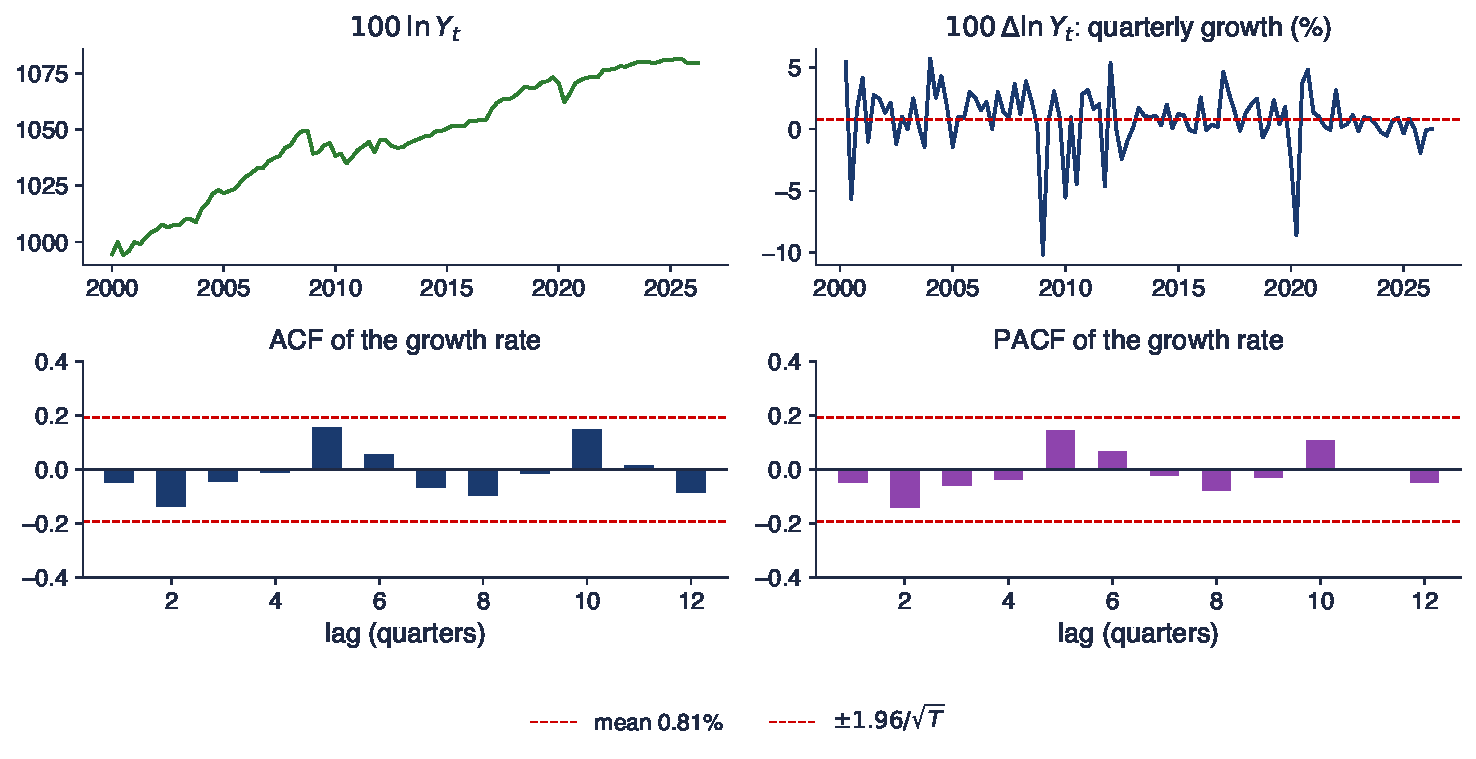
\includegraphics[width=0.97\textwidth,height=0.66\textheight,keepaspectratio]{tsa_ch3_gdp_ident.pdf}
\end{center}
\vspace{-0.25cm}
\begin{itemize}
    \item Real GDP, seasonally adjusted (Eurostat), 2000Q1--2026Q2, $T = 106$; top: $100\ln Y_t$ and the quarterly growth; bottom: ACF and PACF of the growth
\end{itemize}
\quantlet{TSA\_ch3\_arima\_gdp}{\qlurl{TSA_ch3_arima_gdp}}
\end{frame}

\begin{frame}{Interpreting the identification plots}
\itemsize{\small}
\begin{itemize}
    \item $d = 1$: the level is $I(1)$ (Section 4); the growth rate is stationary, mean 0.81\% per quarter (about 3.2\% per year)
    \begin{itemize}
        \item two large falls: \ensuremath{-}10.2\% in 2009Q1 (global financial crisis) and \ensuremath{-}8.6\% in 2020Q2 (pandemic)
    \end{itemize}
    \item $p$ and $q$: no ACF or PACF value outside $\pm 0.19$; $\hat\rho(1) = \ensuremath{-}0.05$, $\hat\rho(2) = \ensuremath{-}0.14$
    \begin{itemize}
        \item Ljung--Box $Q^*(8) = 7.3$ (p = 0.51): the growth rate looks like white noise around its mean
    \end{itemize}
    \item The plots suggest ARIMA(0,1,0) with drift; the next slide checks the alternatives
\end{itemize}
\end{frame}

\begin{frame}{Model choice by AICc}
\itemsize{\small}
\begin{center}
\footnotesize
\begin{tabular}{lccc}
\toprule
& $q = 0$ & $q = 1$ & $q = 2$ \\
\midrule
$p = 0$ & 491.9 & 493.7 & 493.6 \\
$p = 1$ & 493.8 & 494.9 & 495.8 \\
$p = 2$ & 493.7 & 495.7 & 495.4$^\dagger$ \\
\bottomrule
\end{tabular}
\end{center}
\begin{itemize}
    \item ARIMA$(p,1,q)$ with drift for $100\ln Y_t$, estimated by maximum likelihood; AICc: AIC with the small-sample correction (\tsachlink{https://danpele.github.io/Time-Series-Analysis/EN/Courses/chapter2_arma_models.pdf}{Chapter 2}); $^\dagger$: the optimiser did not converge
    \item Lowest AICc: ARIMA(0,1,0); the next model is 1.7 points worse
    \begin{itemize}
        \item differences below 2 points are not meaningful: keep the simplest model
    \end{itemize}
    \item Estimate: drift $\hat c = 0.81$ (SE 0.30, $t = 2.72$), $\hat\sigma = 2.47$: $100\,\Delta\ln Y_t = 0.81 + \hat\varepsilon_t$
\end{itemize}\quantlet{TSA\_ch3\_arima\_gdp}{\qlurl{TSA_ch3_arima_gdp}}
\end{frame}

\begin{frame}{Romanian GDP: residual checks}
\itemsize{\footnotesize}
\begin{center}
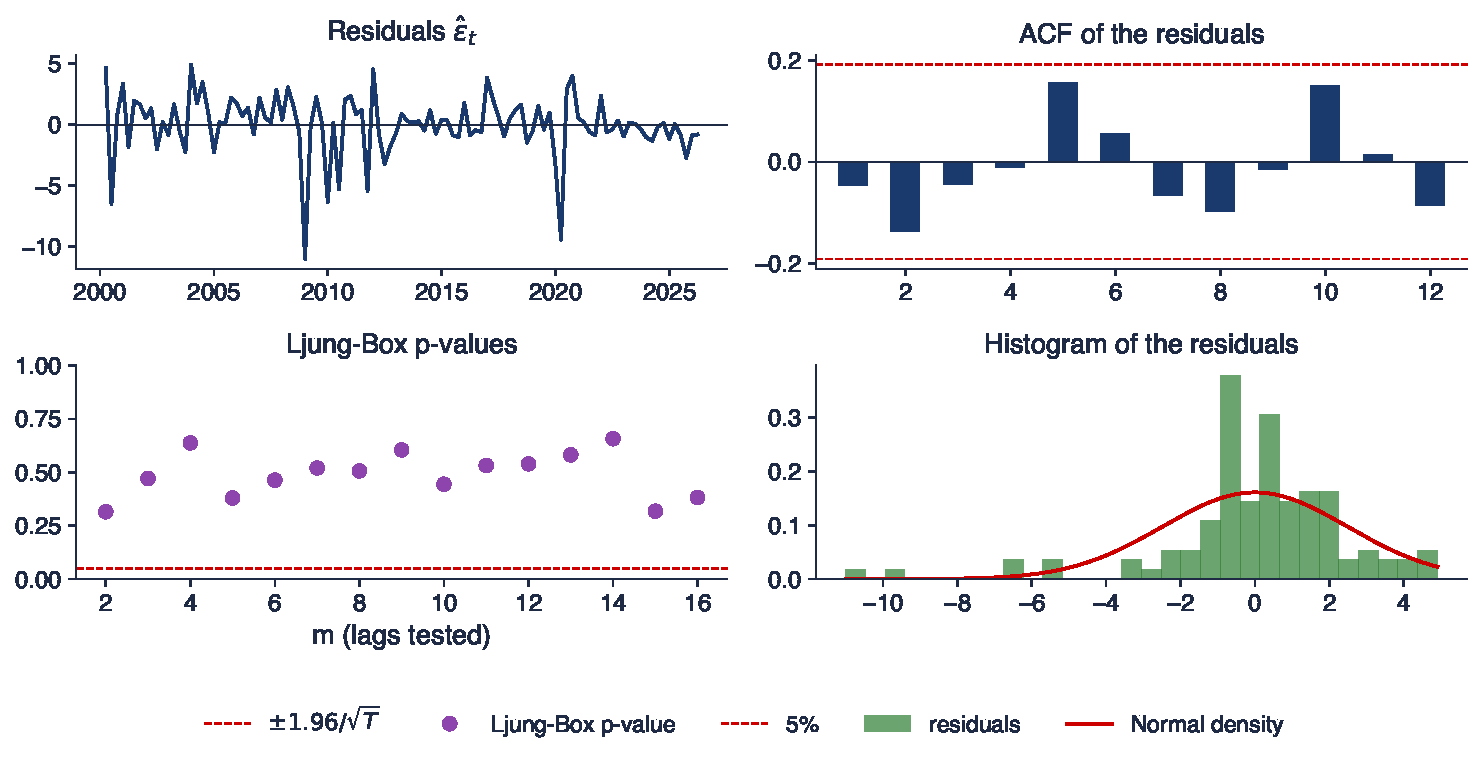
\includegraphics[width=0.97\textwidth,height=0.66\textheight,keepaspectratio]{tsa_ch3_gdp_diag.pdf}
\end{center}
\vspace{-0.25cm}
\begin{itemize}
    \item Residuals of ARIMA(0,1,0) with drift: time plot, ACF, Ljung--Box p-values for $m = 2, \dots, 16$, histogram with a Normal density
\end{itemize}
\quantlet{TSA\_ch3\_arima\_gdp}{\qlurl{TSA_ch3_arima_gdp}}
\end{frame}

\begin{frame}{Interpreting the residual checks}
\itemsize{\small}
\begin{itemize}
    \item No autocorrelation left: $Q^*(8) = 7.3$ (p = 0.51), $Q^*(12)$ p = 0.54; all p-values above 5\%
    \item Not Normal: kurtosis 7.9, Jarque--Bera 145; the largest residual is $\ensuremath{-}11.0$ in 2009Q1
    \begin{itemize}
        \item two crises dominate the tails; the Normal intervals of the next slides are too narrow in a crisis and slightly too wide in calm times
        \item options: dummy variables for 2009 and 2020, or a bootstrap of the residuals for the intervals
    \end{itemize}
\end{itemize}
\end{frame}

\begin{frame}{Forecasting with ARIMA}
\itemsize{\small}
\begin{itemize}
    \item \textbf{Point forecasts}: write the model for the levels and iterate it, with $\hat\varepsilon_{T+j} = 0$ for $j \ge 1$
    \begin{itemize}
        \item ARIMA(1,1,0): $y_t = (1 + \phi)y_{t-1} - \phi y_{t-2} + \varepsilon_t$
    \end{itemize}
    \item \textbf{Forecast error}: $y_{T+h} - \hat y_{T+h} = \sum_{j=0}^{h-1}\psi_j\varepsilon_{T+h-j}$, with $\psi(z) = \theta(z)/[\phi(z)(1 - z)^d]$
    \begin{itemize}
        \item variance $\sigma^2\sum_{j=0}^{h-1}\psi_j^2$; 95\% interval $\hat y_{T+h} \pm 1.96\,\sigma\sqrt{\sum_{j<h}\psi_j^2}$
        \item for $d \ge 1$ the $\psi_j$ do not decay to 0: the variance grows without bound
    \end{itemize}
    \item Two closed forms
    \begin{itemize}
        \item random walk: $\psi_j = 1$, variance $h\sigma^2$: the interval grows like $\sqrt{h}$
        \item ARIMA(0,1,1): $\psi_j = 1 + \theta$ for $j \ge 1$, variance $\sigma^2[1 + (h - 1)(1 + \theta)^2]$
    \end{itemize}
\end{itemize}
\end{frame}

\begin{frame}{Worked example: ARIMA(1,1,0) forecasts}
\itemsize{\small}
\begin{itemize}
    \item $\Delta y_t = 0.6\,\Delta y_{t-1} + \varepsilon_t$, $\sigma = 2$; last data: $y_T = 108$, $\Delta y_T = 5$
    \item \textbf{Point forecasts}: forecast the change, then add it
    \begin{itemize}
        \item $\widehat{\Delta y}_{T+1} = 0.6 \cdot 5 = 3$, $\hat y_{T+1} = 111.00$; $\widehat{\Delta y}_{T+2} = 1.8$, $\hat y_{T+2} = 112.80$; $\hat y_{T+3} = 113.88$
    \end{itemize}
    \item \textbf{$\psi$ weights}: $\psi_0 = 1$, $\psi_1 = 1 + \phi = 1.60$, $\psi_2 = 1 + \phi + \phi^2 = 1.96$
    \begin{itemize}
        \item variances: $4$, $4(1 + 1.60^2) = 14.24$, $4(1 + 1.60^2 + 1.96^2) = 29.61$
        \item 95\% half-widths: 3.92, 7.40, 10.66: the interval almost triples in three steps
    \end{itemize}
    \item The momentum $\phi = 0.6$ makes the uncertainty grow faster than for a random walk ($\sqrt{3} = 1.73$ times in three steps)
\end{itemize}
\end{frame}

\begin{frame}{How fast the intervals grow}
\itemsize{\footnotesize}
\begin{center}
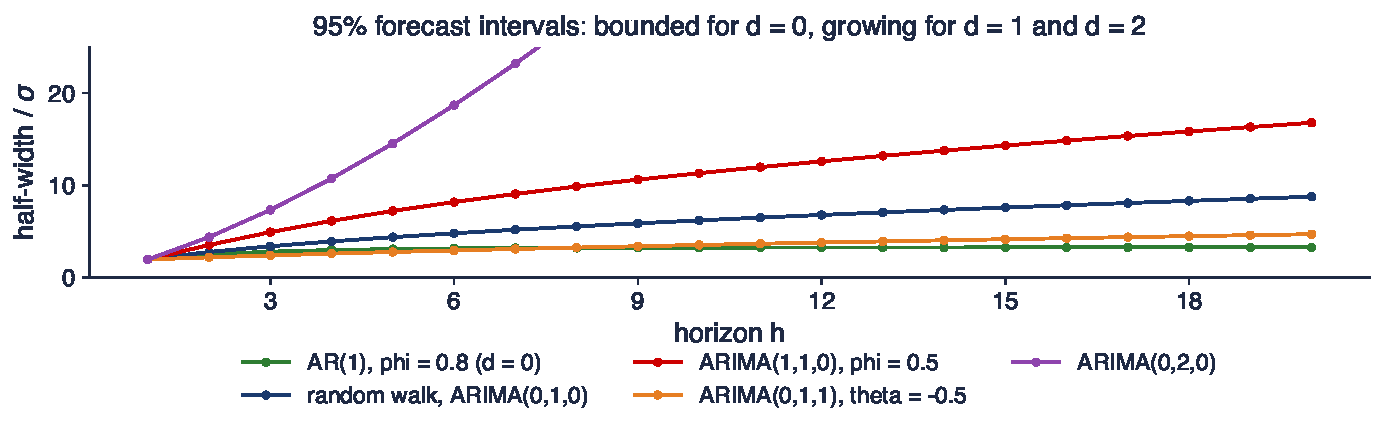
\includegraphics[width=0.97\textwidth,height=0.56\textheight,keepaspectratio]{tsa_ch3_interval_width.pdf}
\end{center}
\vspace{-0.25cm}
\begin{itemize}
    \item Half-width of the 95\% forecast interval, in units of $\sigma$, for horizons 1 to 20, from the $\psi$ weights of five models
\end{itemize}
\quantlet{TSA\_ch3\_forecast\_intervals}{\qlurl{TSA_ch3_forecast_intervals}}
\end{frame}

\begin{frame}{Interpreting the interval widths}
\itemsize{\small}
\begin{itemize}
    \item $d = 0$, AR(1) with $\phi = 0.8$: the width levels off at $1.96\sigma/\sqrt{1 - \phi^2}$ (3.27$\sigma$ at $h = 20$)
    \item $d = 1$: growth like $\sqrt{h}$; at $h = 20$: 8.77$\sigma$ (random walk), 16.78$\sigma$ (ARIMA(1,1,0)), 4.70$\sigma$ (ARIMA(0,1,1), $\theta = -0.5$)
    \begin{itemize}
        \item a negative MA part offsets part of each shock: narrower intervals
    \end{itemize}
    \item $d = 2$: growth like $h^{3/2}$ (105.00$\sigma$ at $h = 20$): over-differencing makes long-run forecasts useless
\end{itemize}
\end{frame}

\begin{frame}{Romanian GDP: two forecasts}
\itemsize{\footnotesize}
\begin{center}
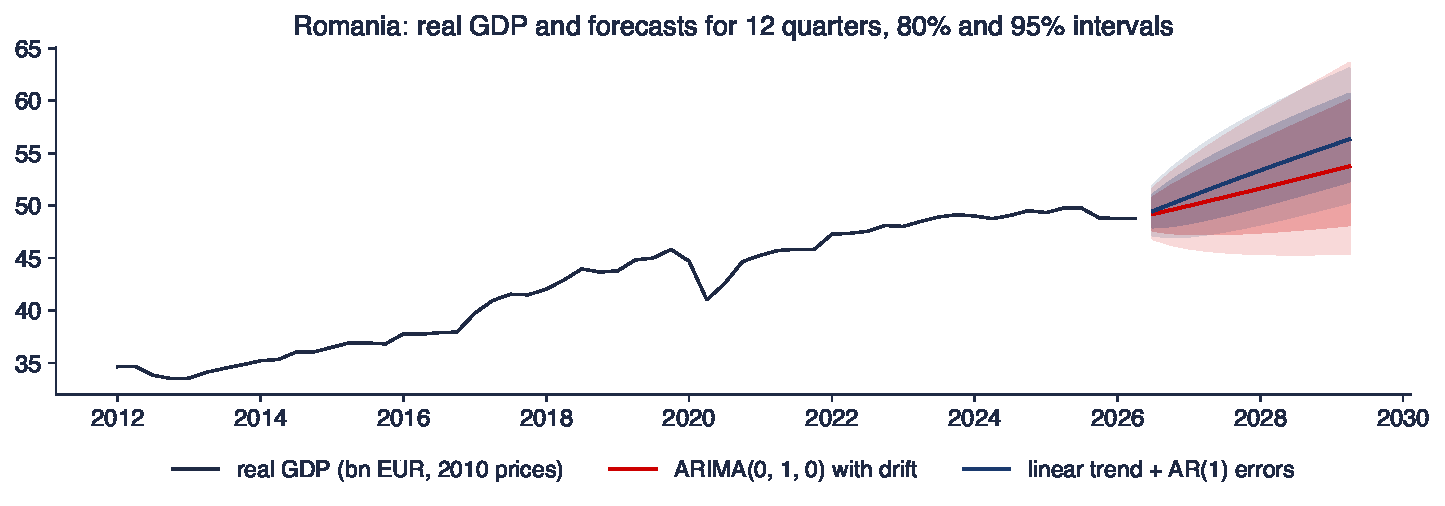
\includegraphics[width=0.97\textwidth,height=0.56\textheight,keepaspectratio]{tsa_ch3_gdp_forecast.pdf}
\end{center}
\vspace{-0.25cm}
\begin{itemize}
    \item ARIMA(0,1,0) with drift (red) and a linear trend with AR(1) errors (blue), both estimated on 2000Q1--2026Q2; forecasts to 2029Q2, transformed back to bn EUR
\end{itemize}
\quantlet{TSA\_ch3\_arima\_gdp}{\qlurl{TSA_ch3_arima_gdp}}
\end{frame}

\begin{frame}{Interpreting the GDP forecasts}
\itemsize{\small}
\begin{itemize}
    \item The random walk with drift grows by 0.81\% per quarter from the last value (48.8 bn EUR in 2026Q2): 53.8 bn after 12 quarters
    \begin{itemize}
        \item 95\% half-width (in \% of GDP): 4.8 after 1 quarter, 9.7 after 4, 16.8 after 12, i.e.\ $\times$3.46 $= \sqrt{12}$
    \end{itemize}
    \item The TS model pulls GDP back towards its old line ($\hat\phi = 0.92$): 56.3 bn after 12 quarters, half-width 11.2\%
    \begin{itemize}
        \item more optimistic and more confident, because it assumes the recent slowdown is temporary
    \end{itemize}
    \item The tests could not settle TS against DS for this sample: the choice of $d$ is a forecasting decision with consequences
\end{itemize}
\end{frame}

\begin{frame}{Over-differencing}
\itemsize{\small}
\begin{itemize}
    \item Differencing an $I(0)$ series creates an MA unit root: $\Delta\varepsilon_t = \varepsilon_t - \varepsilon_{t-1}$, $\theta = -1$ (\tsachlink{https://danpele.github.io/Time-Series-Analysis/EN/Courses/chapter1_stochastic_processes_stationarity.pdf}{Chapter 1})
    \begin{itemize}
        \item the result is not invertible: no AR($\infty$) representation, poor estimation \refPS
    \end{itemize}
    \item Symptoms
    \begin{itemize}
        \item $\hat\rho(1)$ of the differenced series close to $-0.5$
        \item the variance increases after differencing instead of decreasing
        \item an estimated MA coefficient close to $-1$
    \end{itemize}
    \item Rule: difference only as long as the variance goes down and the tests ask for it
\end{itemize}
\end{frame}

\begin{frame}{Over-differencing Romanian GDP}
\itemsize{\footnotesize}
\begin{center}
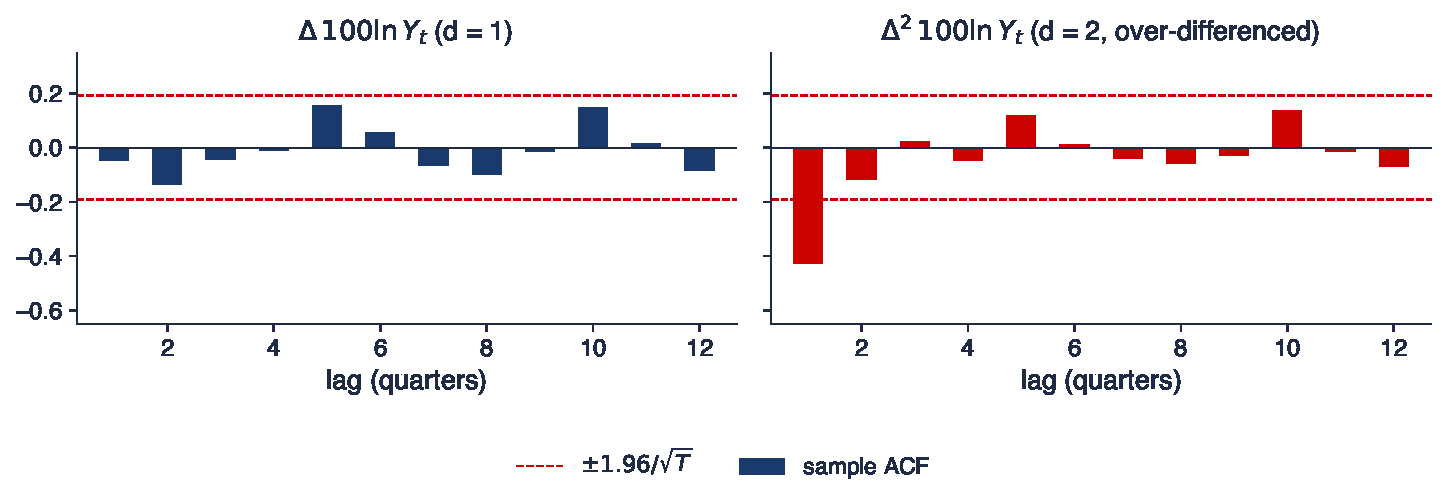
\includegraphics[width=0.97\textwidth,height=0.48\textheight,keepaspectratio]{tsa_ch3_overdiff_gdp.pdf}
\end{center}
\vspace{-0.25cm}
\begin{itemize}
    \item ACF of the quarterly growth $\Delta\,100\ln Y_t$ ($d = 1$) and of its difference $\Delta^2\,100\ln Y_t$ ($d = 2$)
\end{itemize}
\quantlet{TSA\_ch3\_arima\_gdp}{\qlurl{TSA_ch3_arima_gdp}}
\end{frame}

\begin{frame}{Interpreting over-differencing}
\itemsize{\small}
\begin{itemize}
    \item $d = 1$: $\hat\rho(1) = \ensuremath{-}0.05$, variance 6.16; $d = 2$: $\hat\rho(1) = \ensuremath{-}0.43$, variance 12.80: all three symptoms
    \item An MA(1) fitted to $\Delta^2\,100\ln Y_t$ gives $\hat\theta = \ensuremath{-}0.987$ (SE 0.080): practically $-1$, the extra difference is cancelled by the MA part
    \item Correct choice: $d = 1$
\end{itemize}
\end{frame}

\begin{frame}{Recap: ARIMA models}
\itemsize{\small}
\begin{itemize}
    \item ARIMA$(p,d,q)$: an ARMA$(p,q)$ for $\Delta^d y_t$; the constant decides the long-run slope
    \item Romanian GDP since 2000: ARIMA(0,1,0) with drift, 0.81\% per quarter; residuals uncorrelated but heavy-tailed
    \item Forecast variance $\sigma^2\sum_{j<h}\psi_j^2$: bounded for $d = 0$, growing for $d \ge 1$
    \item Over-differencing: $\hat\rho(1) \approx -0.5$, larger variance, MA coefficient near $-1$
\end{itemize}
\end{frame}


%=============================================================================
\section{ARIMA in practice}
%=============================================================================

\begin{frame}{Automatic ARIMA}
\itemsize{\small}
\begin{itemize}
    \item \refHK\ (\texttt{auto.arima} in R; \texttt{pmdarima} and \texttt{statsforecast} in Python):
    \begin{itemize}
        \item $d$: repeated KPSS tests at 5\%: difference while KPSS rejects
        \item $p$, $q$: a stepwise search from a few starting models, by AICc, on the chosen $d$; a constant or drift if $d \le 1$
        \item rejects models with roots too close to the unit circle and fits that fail
    \end{itemize}
    \item Useful for many series at once and as a starting point
    \begin{itemize}
        \item evaluated by its authors on the 3\,003 series of the M3 forecasting competition, it was competitive with the best methods there
    \end{itemize}
    \item But each step embeds a choice that you must be able to defend (next slide)
\end{itemize}
\end{frame}

\begin{frame}{Automatic ARIMA: checks}
\itemsize{\small}
\begin{itemize}
    \item \textbf{AICc is not comparable across $d$}: with $d = 1$ the likelihood is computed for $\Delta y_t$, a different series
    \begin{itemize}
        \item choose $d$ by tests and judgement, then compare $p$, $q$
    \end{itemize}
    \item \textbf{Near-cancelling roots}: Romanian GDP from 1995Q1: the lowest AICc, 607.5 (ARIMA(0,1,0): 611.1), belongs to ARIMA(2,1,2), whose fit did not converge
    \begin{itemize}
        \item MA roots of modulus 1.0002, AR roots 1.014: AR and MA almost cancel; $\hat\theta_2 = 1.000$ with SE 6.96
        \item a model fitted to the noise of the 1990s data, not a description of the economy
    \end{itemize}
    \item \textbf{Always}: plot the data, check the convergence and the roots, run the residual tests, compare with a simple benchmark (random walk, \tsachlink{https://danpele.github.io/Time-Series-Analysis/EN/Courses/chapter0_introduction.pdf}{Chapter 0})
\end{itemize}
\end{frame}

\begin{frame}{Romanian inflation: $d = 0$ or $d = 1$?}
\itemsize{\footnotesize}
\begin{center}
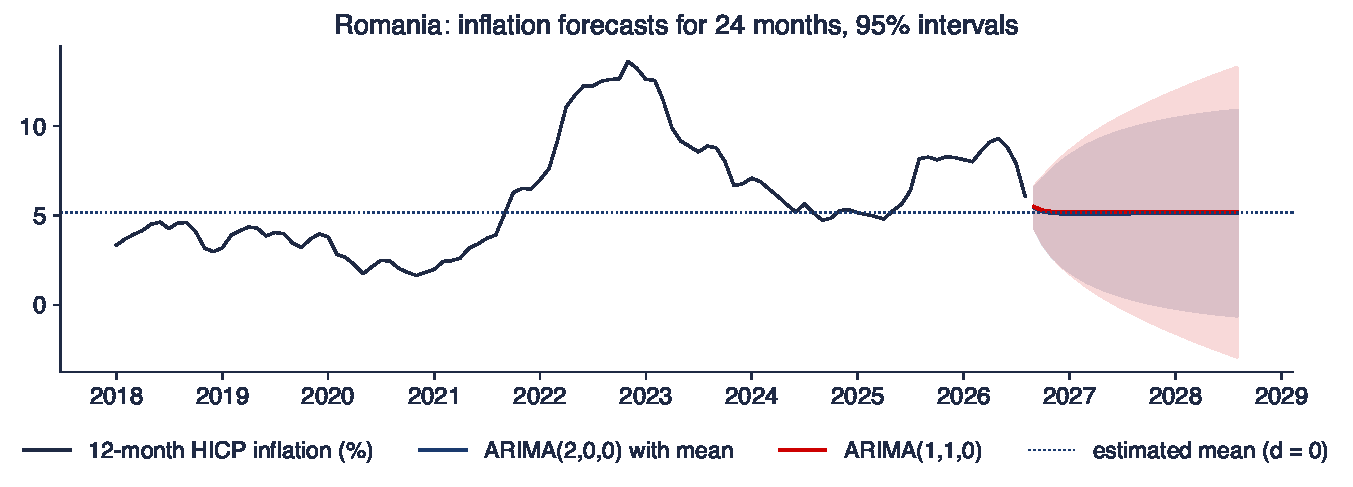
\includegraphics[width=0.97\textwidth,height=0.54\textheight,keepaspectratio]{tsa_ch3_inflation_d.pdf}
\end{center}
\vspace{-0.25cm}
\begin{itemize}
    \item 12-month HICP inflation (Eurostat), January 2005--August 2026; best model by AICc for $d = 0$ (with a mean) and for $d = 1$, $p \le 3$, $q \le 2$; forecasts for 24 months
\end{itemize}
\quantlet{TSA\_ch3\_arima\_in\_practice}{\qlurl{TSA_ch3_arima_in_practice}}
\end{frame}

\begin{frame}{Interpreting the two inflation models}
\itemsize{\small}
\begin{itemize}
    \item $d = 0$: ARIMA(2,0,0), $\hat\phi_1 = 1.32$, $\hat\phi_2 = \ensuremath{-}0.34$, sum 0.976: stationary, but barely; mean 5.2\%
    \begin{itemize}
        \item $d = 1$: ARIMA(1,1,0), $\hat\phi = 0.33$: almost the same short-run dynamics
    \end{itemize}
    \item After 24 months: 5.1\% in $[\ensuremath{-}0.6, 10.9]$ against 5.2\% in $[\ensuremath{-}2.9, 13.3]$
    \begin{itemize}
        \item similar points, different intervals: $d$ decides how much uncertainty we report
    \end{itemize}
    \item KPSS (0.404) keeps $d = 0$, as automatic ARIMA would; ADF (p = 0.32) suggests $d = 1$
    \begin{itemize}
        \item both models leave autocorrelated residuals: 12-month rates overlap and inherit the season; \tsachlink{https://danpele.github.io/Time-Series-Analysis/EN/Courses/chapter4_seasonality_forecasting.pdf}{Chapter 4} models monthly inflation
    \end{itemize}
\end{itemize}
\end{frame}

\begin{frame}{Case study: Meese and Rogoff (1983)}
\itemsize{\small}
\begin{itemize}
    \item \textbf{Question}: can exchange-rate models forecast better than a random walk?
    \begin{itemize}
        \item \refMR: monetary models of the 1970s, time series models (ARIMA, VAR) and the random walk; dollar rates, horizons of 1 to 12 months
    \end{itemize}
    \item \textbf{Finding}: out of sample, none beat the random walk in RMSE (root mean squared error)
    \begin{itemize}
        \item even with the actual future values of the fundamentals plugged in
    \end{itemize}
    \item \textbf{Legacy}: the ``Meese--Rogoff puzzle'' and the random walk as the benchmark for every exchange-rate forecast
    \begin{itemize}
        \item next chart: the same comparison for EUR/RON
    \end{itemize}
\end{itemize}
\end{frame}

\begin{frame}{EUR/RON: ARIMA against the random walk}
\itemsize{\footnotesize}
\begin{center}
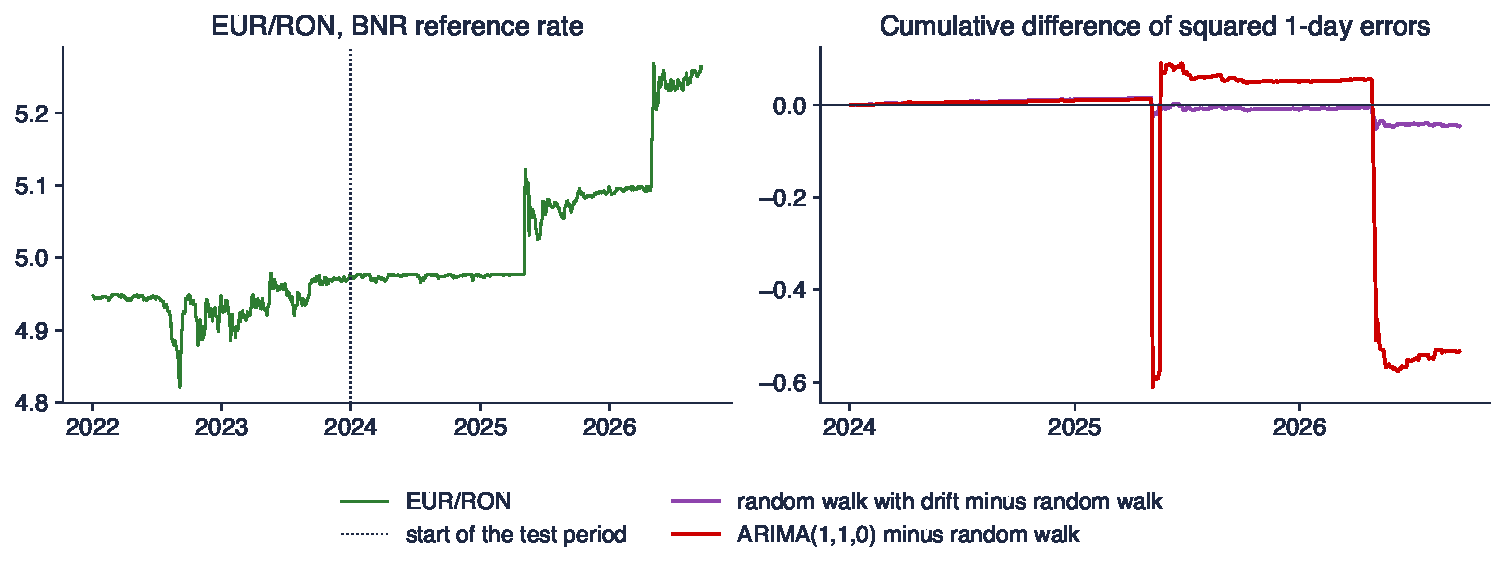
\includegraphics[width=0.97\textwidth,height=0.52\textheight,keepaspectratio]{tsa_ch3_eurron_forecast.pdf}
\end{center}
\vspace{-0.25cm}
\begin{itemize}
    \item Parameters estimated on 4\,673 daily changes until December 2023; 679 one-day-ahead forecasts from January 2024; right: the cumulated difference of squared errors (below 0: the model beats the random walk)
\end{itemize}
\quantlet{TSA\_ch3\_arima\_in\_practice}{\qlurl{TSA_ch3_arima_in_practice}}
\end{frame}

\begin{frame}{Interpreting the EUR/RON comparison}
\itemsize{\small}
\begin{itemize}
    \item RMSE of the daily change ($100\ln$): random walk 0.1330, with drift 0.1327, ARIMA(1,1,0) 0.1300 ($\hat\phi = 0.169$)
    \begin{itemize}
        \item a gain of 2.2\%; over 20 days (33 non-overlapping windows): 0.667 against 0.638, a gain of 4.3\%
    \end{itemize}
    \item The gain comes from a few days: two jumps of the rate (from 4.9746 to 5.2644 lei over the period) continued on the next day
    \begin{itemize}
        \item on calm days the random walk is as good; a formal comparison needs the Diebold--Mariano test (\tsachlink{https://danpele.github.io/Time-Series-Analysis/EN/Courses/chapter4_seasonality_forecasting.pdf}{Chapter 4})
    \end{itemize}
    \item Lesson of Meese and Rogoff: report the random walk next to any exchange-rate forecast
\end{itemize}
\end{frame}

\begin{frame}{A classic series: US real GDP after 2007}
\itemsize{\footnotesize}
\begin{center}
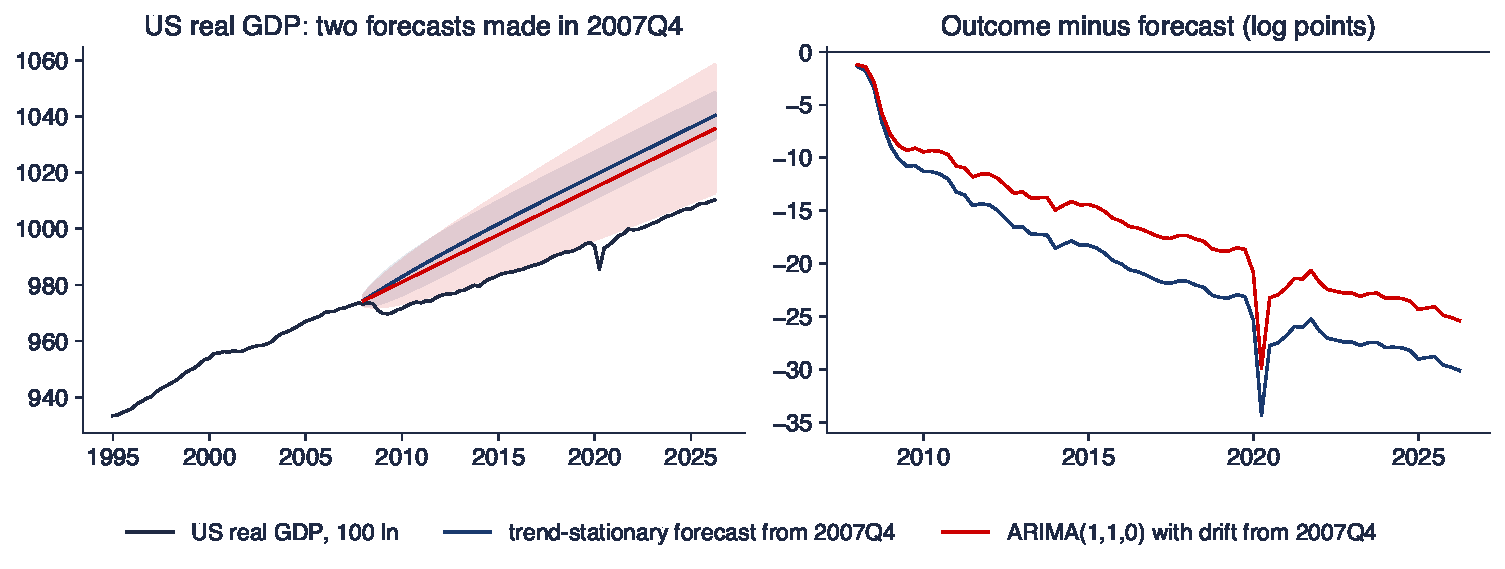
\includegraphics[width=0.97\textwidth,height=0.54\textheight,keepaspectratio]{tsa_ch3_us_gdp.pdf}
\end{center}
\vspace{-0.25cm}
\begin{itemize}
    \item FRED series GDPC1 since 1947; a TS model (linear trend, AR(2) errors) and a DS model (ARIMA(1,1,0) with drift) estimated up to 2007Q4 and forecast to 2026Q2; 95\% intervals
\end{itemize}
\quantlet{TSA\_ch3\_us\_gdp}{\qlurl{TSA_ch3_us_gdp}}
\end{frame}

\begin{frame}{Interpreting the US GDP forecasts}
\itemsize{\small}
\begin{itemize}
    \item The TS model expected a return to the pre-2008 line; the gap kept widening: $\ensuremath{-}30$ log points at the end (half-width of its interval: 8)
    \begin{itemize}
        \item the 2008--2009 loss was never recovered: evidence for a permanent shock, as the DS view of \refNP\ implies
    \end{itemize}
    \item The DS model also misses ($\ensuremath{-}25$), but its interval (half-width 23) at least warns of large uncertainty
    \begin{itemize}
        \item both assume the same drift as before 2008; growth after 2008 was slower: a break in the drift (Section 5)
    \end{itemize}
    \item Unit-root tests on the full series: ADF p = 0.82, KPSS 0.58: $I(1)$
\end{itemize}
\end{frame}

\begin{frame}{Recap: ARIMA in practice}
\itemsize{\small}
\begin{itemize}
    \item Automatic ARIMA: KPSS for $d$, AICc for $p$, $q$; check convergence, roots and residuals
    \item AICc compares models with the same $d$ only
    \item Exchange rates: the random walk is a hard benchmark \refMR
    \item TS or DS changes the long-run forecast and its interval: US GDP after 2008
\end{itemize}
\end{frame}


%=============================================================================
\section{Possible contribution of AI}
%=============================================================================

\begin{frame}{Possible contribution of AI}
\itemsize{\small}
\begin{itemize}
    \item \textbf{Code}: a first draft of a script that runs ADF, PP and KPSS on many series and tabulates the verdicts
    \item \textbf{Explanation}: a second explanation of why the Dickey--Fuller distribution is not Normal, or of a ZA output
    \item \textbf{Exploration}: unit roots and breaks in all EU inflation rates, or ARIMA benchmarks for many Romanian series
    \item Example prompt
    \begin{itemize}
        \item \aiprompt{Write Python code that loads Romanian quarterly real GDP (Eurostat namq\_10\_gdp, seasonally adjusted), runs ADF with constant and trend and KPSS on 100*log GDP and on its difference, fits ARIMA(p,1,q) with drift for p, q <= 2, and plots 8-quarter forecasts with 95\% intervals.}
    \end{itemize}
\end{itemize}
\end{frame}

\begin{frame}{Checks you must run}
\itemsize{\small}
\begin{itemize}
    \item The direction of each test: ADF and PP have the unit root as $H_0$, KPSS has stationarity as $H_0$
    \item The deterministic terms, the number of lags and the critical values actually used (Dickey--Fuller, not Normal)
    \item That ``not rejected'' is not reported as ``proved''
    \item That regressions between trending series are not presented as causal evidence
    \item Convergence warnings, roots near the unit circle, residual tests, and AICc compared only for the same $d$
    \item Every cited reference: it must exist; check the DOI
\end{itemize}
\end{frame}


%=============================================================================
\section{Summary}
%=============================================================================

\begin{frame}{Key takeaways}
\itemsize{\small}
\begin{itemize}
    \item Trending series are TS (shocks fade) or DS (shocks are permanent); the treatment differs: detrend or difference
    \item Regressions between unrelated $I(1)$ series are spurious: high $t$ and $R^2$, DW near 0
    \item ADF and PP test $H_0$: unit root with Dickey--Fuller critical values; KPSS tests $H_0$: stationarity; use them together
    \item The tests have low power near $\phi = 1$ and are misled by breaks; Zivot--Andrews allows one break
    \item ARIMA$(p,d,q)$ = ARMA on $\Delta^d y_t$; its forecast intervals grow with the horizon when $d \ge 1$
    \item Automatic selection is a starting point: check $d$, convergence, roots, residuals and a random-walk benchmark
\end{itemize}
\end{frame}

\begin{frame}{Key formulas}
\itemsize{\small}
{\renewcommand{\arraystretch}{1.4}\begin{center}
\scriptsize
\begin{tabular}{ll}
\toprule
\textbf{Quantity} & \textbf{Formula} \\
\midrule
TS and DS & $y_t = \alpha + \beta t + u_t$, \quad $\Delta y_t = \beta + u_t$, \quad $u_t \sim I(0)$ \\
ADF & $\Delta y_t = c + bt + \gamma y_{t-1} + \sum_{j=1}^{k}\delta_j\Delta y_{t-j} + \varepsilon_t$, \quad $H_0$: $\gamma = 0$, \quad $\tau = \hat\gamma/\mathrm{SE}(\hat\gamma)$ \\
Lags & $k_{\max} = 12\,(T/100)^{1/4}$, then AIC or BIC \\
KPSS & $\eta = \sum_{t=1}^{T} S_t^2/(T^2\hat\lambda^2)$, \quad $S_t = \sum_{s \le t} e_s$, \quad 5\%: 0.463 (c), 0.146 (c, t) \\
ARIMA$(p,d,q)$ & $\phi(L)(1 - L)^d y_t = c + \theta(L)\varepsilon_t$ \\
Forecast variance & $\sigma^2\sum_{j=0}^{h-1}\psi_j^2$, \quad $\psi(z) = \theta(z)/[\phi(z)(1 - z)^d]$; random walk: $h\sigma^2$ \\
ARIMA(0,1,1) & $\sigma^2[1 + (h - 1)(1 + \theta)^2]$, \quad $\alpha_{\mathrm{SES}} = 1 + \theta$ \\
\bottomrule
\end{tabular}
\end{center}
}
\end{frame}

\begin{frame}{Self-assessment}
\itemsize{\small}
\begin{itemize}
    \item \textbf{Question}: an ADF test with constant and trend gives $\tau = -2.9$ with $T = 200$. Do you reject the unit root at 5\%?
    \begin{itemize}
        \item \textbf{Answer}: no: $-2.9 > -3.43$; with the Normal table you would wrongly reject
    \end{itemize}
    \item \textbf{Question}: ADF does not reject and KPSS does not reject. What do you conclude?
    \begin{itemize}
        \item \textbf{Answer}: inconclusive: the sample is too short to decide; report both models, or choose $d$ by the purpose
    \end{itemize}
    \item \textbf{Question}: for ARIMA(0,1,1) with $\theta = -0.6$ and $\sigma = 1$, what is the variance of the 5-step forecast error?
    \begin{itemize}
        \item \textbf{Answer}: $1 + 4 \cdot 0.4^2 = 1.64$
    \end{itemize}
    \item Next: \tsachlink{https://danpele.github.io/Time-Series-Analysis/EN/Courses/chapter4_seasonality_forecasting.pdf}{Chapter 4}, seasonality: seasonal differences, SARIMA, TBATS and Prophet
\end{itemize}
\end{frame}


%=============================================================================
\section{References}
%=============================================================================

\begin{frame}{References (1/3)}
\itemsize{\scriptsize}
\begin{itemize}
    \item Bai, J., \& Perron, P. (1998). Estimating and testing linear models with multiple structural changes. \textit{Econometrica}, 66(1), 47--78. \href{https://doi.org/10.2307/2998540}{doi:10.2307/2998540}
    \item Box, G. E. P., Jenkins, G. M., \& Reinsel, G. C. (2008). \textit{Time Series Analysis: Forecasting and Control} (4th ed.). Wiley. \href{https://doi.org/10.1002/9781118619193}{doi:10.1002/9781118619193}
    \item Brockwell, P. J., \& Davis, R. A. (2016). \textit{Introduction to Time Series and Forecasting} (3rd ed.). Springer. \href{https://doi.org/10.1007/978-3-319-29854-2}{doi:10.1007/978-3-319-29854-2}
    \item Dickey, D. A., \& Fuller, W. A. (1979). Distribution of the estimators for autoregressive time series with a unit root. \textit{Journal of the American Statistical Association}, 74(366), 427--431. \href{https://doi.org/10.1080/01621459.1979.10482531}{doi:10.1080/01621459.1979.10482531}
    \item Dickey, D. A., \& Fuller, W. A. (1981). Likelihood ratio statistics for autoregressive time series with a unit root. \textit{Econometrica}, 49(4), 1057--1072. \href{https://doi.org/10.2307/1912517}{doi:10.2307/1912517}
    \item Dickey, D. A., \& Pantula, S. G. (1987). Determining the order of differencing in autoregressive processes. \textit{Journal of Business \& Economic Statistics}, 5(4), 455--461. \href{https://doi.org/10.1080/07350015.1987.10509614}{doi:10.1080/07350015.1987.10509614}
    \item Elliott, G., Rothenberg, T. J., \& Stock, J. H. (1996). Efficient tests for an autoregressive unit root. \textit{Econometrica}, 64(4), 813--836. \href{https://doi.org/10.2307/2171846}{doi:10.2307/2171846}
    \item Engle, R. F., \& Granger, C. W. J. (1987). Co-integration and error correction: Representation, estimation, and testing. \textit{Econometrica}, 55(2), 251--276. \href{https://doi.org/10.2307/1913236}{doi:10.2307/1913236}
    \item Fuller, W. A. (1996). \textit{Introduction to Statistical Time Series} (2nd ed.). Wiley. \href{https://doi.org/10.1002/9780470316917}{doi:10.1002/9780470316917}
    \item Granger, C. W. J., \& Newbold, P. (1974). Spurious regressions in econometrics. \textit{Journal of Econometrics}, 2(2), 111--120. \href{https://doi.org/10.1016/0304-4076(74)90034-7}{doi:10.1016/0304-4076(74)90034-7}
\end{itemize}
\end{frame}

\begin{frame}{References (2/3)}
\itemsize{\scriptsize}
\begin{itemize}
    \item Hamilton, J. D. (1994). \textit{Time Series Analysis}. Princeton University Press. \href{https://doi.org/10.2307/j.ctv14jx6sm}{doi:10.2307/j.ctv14jx6sm}
    \item Huang, C., \& Petukhina, A. (2022). \textit{Applied Time Series Analysis and Forecasting with Python}. Springer. \href{https://doi.org/10.1007/978-3-031-13584-2}{doi:10.1007/978-3-031-13584-2}
    \item Hyndman, R. J., \& Athanasopoulos, G. (2021). \textit{Forecasting: Principles and Practice} (3rd ed.). OTexts. \href{https://otexts.com/fpp3/}{otexts.com/fpp3}
    \item Hyndman, R. J., \& Khandakar, Y. (2008). Automatic time series forecasting: The forecast package for R. \textit{Journal of Statistical Software}, 27(3), 1--22. \href{https://doi.org/10.18637/jss.v027.i03}{doi:10.18637/jss.v027.i03}
    \item Kwiatkowski, D., Phillips, P. C. B., Schmidt, P., \& Shin, Y. (1992). Testing the null hypothesis of stationarity against the alternative of a unit root. \textit{Journal of Econometrics}, 54(1--3), 159--178. \href{https://doi.org/10.1016/0304-4076(92)90104-Y}{doi:10.1016/0304-4076(92)90104-Y}
    \item Ljung, G. M., \& Box, G. E. P. (1978). On a measure of lack of fit in time series models. \textit{Biometrika}, 65(2), 297--303. \href{https://doi.org/10.1093/biomet/65.2.297}{doi:10.1093/biomet/65.2.297}
    \item MacKinnon, J. G. (1994). Approximate asymptotic distribution functions for unit-root and cointegration tests. \textit{Journal of Business \& Economic Statistics}, 12(2), 167--176. \href{https://doi.org/10.1080/07350015.1994.10510005}{doi:10.1080/07350015.1994.10510005}
    \item MacKinnon, J. G. (2010). Critical values for cointegration tests. Queen's Economics Department Working Paper No.~1227, Queen's University. \href{https://ideas.repec.org/p/qed/wpaper/1227.html}{ideas.repec.org/p/qed/wpaper/1227}
    \item Meese, R. A., \& Rogoff, K. (1983). Empirical exchange rate models of the seventies: Do they fit out of sample? \textit{Journal of International Economics}, 14(1--2), 3--24. \href{https://doi.org/10.1016/0022-1996(83)90017-X}{doi:10.1016/0022-1996(83)90017-X}
    \item Nelson, C. R., \& Kang, H. (1981). Spurious periodicity in inappropriately detrended time series. \textit{Econometrica}, 49(3), 741--751. \href{https://doi.org/10.2307/1911520}{doi:10.2307/1911520}
\end{itemize}
\end{frame}

\begin{frame}{References (3/3)}
\itemsize{\scriptsize}
\begin{itemize}
    \item Nelson, C. R., \& Plosser, C. I. (1982). Trends and random walks in macroeconomic time series: Some evidence and implications. \textit{Journal of Monetary Economics}, 10(2), 139--162. \href{https://doi.org/10.1016/0304-3932(82)90012-5}{doi:10.1016/0304-3932(82)90012-5}
    \item Ng, S., \& Perron, P. (2001). Lag length selection and the construction of unit root tests with good size and power. \textit{Econometrica}, 69(6), 1519--1554. \href{https://doi.org/10.1111/1468-0262.00256}{doi:10.1111/1468-0262.00256}
    \item Perron, P. (1989). The Great Crash, the oil price shock, and the unit root hypothesis. \textit{Econometrica}, 57(6), 1361--1401. \href{https://doi.org/10.2307/1913712}{doi:10.2307/1913712}
    \item Phillips, P. C. B. (1986). Understanding spurious regressions in econometrics. \textit{Journal of Econometrics}, 33(3), 311--340. \href{https://doi.org/10.1016/0304-4076(86)90001-1}{doi:10.1016/0304-4076(86)90001-1}
    \item Phillips, P. C. B., \& Perron, P. (1988). Testing for a unit root in time series regression. \textit{Biometrika}, 75(2), 335--346. \href{https://doi.org/10.1093/biomet/75.2.335}{doi:10.1093/biomet/75.2.335}
    \item Plosser, C. I., \& Schwert, G. W. (1977). Estimation of a non-invertible moving average process: The case of overdifferencing. \textit{Journal of Econometrics}, 6(2), 199--224. \href{https://doi.org/10.1016/0304-4076(77)90015-x}{doi:10.1016/0304-4076(77)90015-x}
    \item Said, S. E., \& Dickey, D. A. (1984). Testing for unit roots in autoregressive-moving average models of unknown order. \textit{Biometrika}, 71(3), 599--607. \href{https://doi.org/10.1093/biomet/71.3.599}{doi:10.1093/biomet/71.3.599}
    \item Schwert, G. W. (1989). Tests for unit roots: A Monte Carlo investigation. \textit{Journal of Business \& Economic Statistics}, 7(2), 147--159. \href{https://doi.org/10.1080/07350015.1989.10509723}{doi:10.1080/07350015.1989.10509723}
    \item Yule, G. U. (1926). Why do we sometimes get nonsense-correlations between time-series? A study in sampling and the nature of time-series. \textit{Journal of the Royal Statistical Society}, 89(1), 1--63. \href{https://doi.org/10.2307/2341482}{doi:10.2307/2341482}
    \item Zivot, E., \& Andrews, D. W. K. (1992). Further evidence on the Great Crash, the oil-price shock, and the unit-root hypothesis. \textit{Journal of Business \& Economic Statistics}, 10(3), 251--270. \href{https://doi.org/10.1080/07350015.1992.10509904}{doi:10.1080/07350015.1992.10509904}
\end{itemize}
\end{frame}

\end{document}
